



\documentclass[leqno]{book}
\usepackage{amsmath,amssymb,amsthm, amscd}
\usepackage{hyperref}
\usepackage{etoolbox}
\usepackage{everysel}
\usepackage{titlesec}
\usepackage{marginnote}
\usepackage[a4paper, textwidth=39cm, margin=1.1in, vmargin=3cm, marginparsep=20pt, marginparwidth=.6in,]{geometry} 
\usepackage{fancyhdr}
\usepackage{graphicx}
\usepackage{float}
\input macros.tex

%%%%%%%%%%maring notes%%%%%%%%%%
%\usepackage{ragged2e}
%\renewcommand*{\raggedleftmarginnote}{\RaggedLeft}
%\renewcommand*{\raggedrightmarginnote}{\RaggedRight}
\newcommand\Marginnote[1]{\marginnote{\hspace{-12pt}\normalfont{#1}}}

%%%%put all marginnotes to the left margin%%%%%%%%%
\makeatletter
\patchcmd{\@mn@margintest}{\@tempswafalse}{\@tempswatrue}{}{}
\patchcmd{\@mn@margintest}{\@tempswafalse}{\@tempswatrue}{}{}
\reversemarginpar 
\makeatother

%%%%%%Reduce font size of chapter and section%%%%
\usepackage{titlesec}

\titleformat{\section}
  {\normalfont\fontsize{12}{12}\bfseries}{\thesection}{1em}{}

\titleformat{\chapter}
  {\normalfont\fontsize{14}{14}\bfseries}{Chapter \thechapter}{1em}{}

\newcommand{\lsec}{\titleformat{\section}
  {\normalfont\fontsize{12}{12}\bfseries}{Section \thesection}{1em}{}}
 
\setlength{\parskip}{.2em}
\titlespacing*{\section}{0pt}{3ex plus 1ex minus .2ex}{1ex plus .1ex}

\newcommand\secstore{}
\newcommand\mythesection{\arabic{chapter}.}

%%%%%%%%makes equation numbers bold%%%%%%%%%%%%%
\renewcommand\theequation{\thesection.\arabic{equation}}
\newenvironment{boldequation}{\renewcommand\theequation{\textbf{\thesection.\arabic{equation}}}\equation}
   {\endequation}

%%%%%create theroem environment%%%%%%%%
\newtheoremstyle{dotless}{}{}{\itshape}{}{\bfseries}{}{ }{}
\swapnumbers
\theoremstyle{definition}%{no italic}
\numberwithin{equation}{section}
\newtheorem{note}[equation]{}
\newtheorem{definition}[equation]{}
\newtheorem{example}[equation]{}
\newtheorem{examples}[equation]{}
\newtheorem{remarks}[equation]{}
\newtheorem{thm}[equation]{}

\theoremstyle{theorem} %{italic}
\newtheorem{lemma}[equation]{}
\newtheorem{proposition}[equation]{}
\newtheorem{corollary}[equation]{}
\newtheorem{theorem}[equation]{}
\newtheorem{thrm}[equation]{}
 
\renewenvironment{proof}{\no \emph{proof.}}{}

%%%%%%%%Font style%%%%%%%%%
\usepackage[T1]{fontenc}
\usepackage{textcomp}
\renewcommand{\rmdefault}{ptm}
\usepackage[scaled=0.98]{helvet}
 
%%%%%%%%%%%Headers and footers%%%%%%%%%%%%
\pagestyle{fancy}% Set default page style to fancy
\renewcommand{\headrulewidth}{0pt}% Remove header rule
\fancyhead{}% Remove all header contents
\cfoot{\thepage}
 
%%%%%%%%%%%\crossreferences%
\makeatletter
\DeclareRobustCommand*\Cal{\@fontswitch\relax\mathcal}
\makeatother
\usepackage{xr}


     \externaldocument{chap1v65}
     \externaldocument{chap2v43}
     \externaldocument{chap3v51}
     \externaldocument{chap4v49}
     \externaldocument{chap5v54}
     \externaldocument{newchap6v9}
     \externaldocument{newchap7v9}
     \externaldocument{newchap8v3}
%     \externaldocument{chap9v22}

     
\begin{document}


\chapter{PLANE CURVES}\MMM{planecurves} \label{planecurves}
 
\no
version 64
\no


	\ref{affineplane}  \;  {\bf The Affine Plane}  
	
	\ref{projplane} \;  {\bf The Projective Plane} 

        \ref{projcurve} \; {\bf Plane Projective Curves} 

	\ref{tanlines} \;  {\bf Tangent Lines} 
	
	\ref{nodes} \; {\bf  Nodes and Cusps} 
	
	\ref{transcdeg} \;  {\bf Transcendence Degree}
	
	\ref{dualcurve} \;  {\bf  The Dual Curve}

	\ref{resultant} \;  {\bf Resultants}
	
	\ref{coverline} \; {\bf  Coverings of the Projective Line}
	
	\ref{genus} \;  {\bf Genus}

	\ref{bezoutthm} \;  {\bf B\'ezout's Theorem} 

       \ref{plucker}  \; {\bf The Pl\"ucker Formulas}

\ms \#\#change coordinates $t,u=t^{-1}$ for $\bbp^1$ to $u,v=u^{-1}$
throughout\#\#

\#\# affine blowing up is only in this chapter
redefined in Chap 3 for projection, not used, i think
\#\#

\bsno Plane curves were the first algebraic varieties to be studied.
They provide examples that are helpful for understanding varieties
of higher dimension, so we begin with them.


\section{The Affine  Plane} 
\label{affineplane} \Marginnote{affineplane}[-.6cm]

\msno The
$n$-dimensional {\it affine space} $\bba^n$ is the space of
$n$-tuples of complex numbers.  The
{\it affine plane} $\bba^2$ is the two-dimensional affine space.


If $f(x_1,x_2)$ is an irreducible polynomial in two variables with
complex coefficients, the set of points $X$ of the affine plane at
which $f$ vanishes, the {\it locus of zeros} of $f$, is called a {\it plane
curve}, or an {\it affine plane curve}.  Using vector notation
  $x=(x_1,x_2)$,
\begin{equation}
X \;=\; \{x \,|\, f(x)=0\}  \Marginnote{affcurve}
	\label{affcurve}
\end{equation}
 
\no
The {\it degree} of the curve $X$ is the degree of its
irreducible defining polynomial. 

$$figure$$



\ms
\begin{note}{\bf Note.}  \Marginnote{polyirred}
In contrast with polynomials in one variable, most complex polynomials
in two or more variables are irreducible -- they cannot be factored.
This can be shown by a method called ``counting constants''.  For
instance, quadratic polynomials in $x_1,x_2$ depend on the
coefficients of the six monomials in $x_1,x_2$ of degree at most two.
Linear polynomials $ax_1\!+\!bx_2\!+\!c$ depend on three coefficients,
but the product of two linear polynomials depends on only five
parameters, because a scalar factor can be moved from one of the
linear polynomials to the other.  So the quadratic polynomials cannot
all be written as products of linear polynomials.  This reasoning is
fairly clear.  It can be justified formally in terms of {\it
  dimension}, which will be discussed in Chapter \ref{zarstr}.\qed
\label{polyirred}\end{note}

As this chapter progresses, we will get some understanding of the
geometry of a plane curve. Here we mention just one important point.
A plane curve is called a curve because it is defined by one
equation in two variables.  Its {\it algebraic} dimension is one.  But
because our scalars are complex numbers, it will be a surface,
geometrically.  This is analogous to the fact that the {\it affine
  line} $\bba^1$ is the plane of complex numbers.

One can see that a plane curve is a surface by inspecting its
projection to the affine line.  To do this, one writes its defining
polynomial $f$ as a polynomial in $x_2$ whose coefficients are
polynomials in $x_1$:
$$f(x_1,x_2) = c_0(x_1)x_2^d + c_1(x_1)x_2^{d-1} + \cdots + c_d(x_1)$$

\no Let's suppose that $f$ isn't a polynomial in $x$ alone, so that
$d$ is positive.  The {\it fibre} of a map $X \ar Z$ over a point $q$
of $Z$ is defined to be the inverse image of $q$, the set of points of
$X$ that map to $q$.  The fibre of the projection $X \ar \bba^1$ over
a point $x_1 = a$ is the set of points $(a,b)$ such that $b$ is a root
of the one-variable polynomial $$f(a,x_2) = c_0(a)x_2^d +
c_1(a)x_2^{d-1} + \cdots + c_d(a)$$ There will be finitely many points
in the fibre, and the fibre won't be empty unless $f(a,x_2)$ is a
constant.  So $X$ covers most of the $x_1$-line, a complex plane,
finitely often.

\begin{boldequation}
\Marginnote{planecoords}\hspace{-9.5cm} \textbf {changing coordinates}
	\label{planecoords}
\end{boldequation}


When classifying plane curves, one allows linear
changes of variable and translations.  If we write $x$ as the column
vector $(x_1,x_2)^t$, the coordinates $x'= (x_1',x_2')^t$ after such a
change of variable will have the form

\begin{equation}
Qx'+a=x \Marginnote{chgcoord}
	\label{chgcoord}
\end{equation}

\no where $Q$ is an invertible $2\times 2$ matrix with complex
coefficients and $a= (a_1,a_2)^t$ is a complex translation vector.
This changes a polynomial equation $f(x)=0$, to $\,f(Qx'+a) = 0$.  One
may also multiply a polynomial $f$ by a (nonzero) complex scalar without
changing the locus $\{f=0\}$.  
Using these operations, all {\it
  lines}, plane curves of degree $1$, become equivalent.


\ms An {\it affine conic} is a plane curve of degree two.  Every equation
$q(x_1,x_2)=0$ in which $q$ is an irreducible quadratic polynomial is
equivalent by a change of coordiantes  to one of the two equations
 
\begin{equation}
x_1^2 - x_2^2 -1=0\quad\text{or}\quad 
x_1^2-x_2=0 
\end{equation} 

\no The proof of this is similar to the one used to classify real conics.
The loci of solutions of the two equations might be called a complex
'hyperbola' and 'parabola', respectively.  The complex 'ellipse'
$x_1^2+x_2^2-1=0$ becomes the hyperbola when one multiplies $x_2$ by
$i$.

 On the other hand, there are infinitely many inequivalent
cubic curves.  Cubic polynomials in two variables depend on the
coefficients of the ten monomials in $x_1,x_2$ of degree at most $3$.
Linear operators, translations, and scalar multiplication give us only
seven parameters to work with, leaving three essential parameters.

 
\section{The Projective Plane}\label{projplane}\Marginnote{projplane}[-.6cm]

 \msno The $n$-dimensional {\it projective space} $\bbp^n$ is the set
 of equivalence classes of {\it nonzero} vectors $x= (x_0,x_1,...,x_n)$,
 the equivalence relation being

\begin{equation}(x_0',...,x_n') \sim (x_0,...,x_n)\;\;\;\;\text{if}\;\;\;\; 
(x_0',...,x_n') = (\lambda x_0,...,\lambda
    x_n)\MMM{equivrel}\label{equivrel}
\end{equation}
 for some nonzero
complex number $\lambda$.  The equivalence classes are the {\it
  points} of $\bbp^n$, and one often refers to a point by a particular
vector in its class.  
 Points of $\bbp^n$  correspond
bijectively to one-dimensional subspaces of $\bbc^{n+1}$.
If $x$ is a nonzero vector, the vectors $\lambda x$, together with the
zero vector, form the one-dimensional subspace of the complex vector
space $\bbc^{n+1}$ spanned by $x$. 

The {\it projective plane} is the two-dimensional projective space.

\begin{boldequation}
\Marginnote{projline}\hspace{-10cm} \textbf {the projective line}
	\label{projline} 
\end{boldequation}


Points of the {projective line} $\bbp^1$ are equivalence classes of
nonzero vectors $(x_0,x_1)$.  If $x_0$ isn't zero, we may multiply by
$\lambda = x_0^{-1}$ to normalize the first entry of a point
$(x_0,x_1)$ to $1$, and write the point it represents in a unique way
as $(1,u)$, with $u=x_1/x_0$.  There is one remaining point, the one
represented by the vector $(0,1)$.  The projective line $\bbp^1$ can
be obtained by adding this point, called the {\it point at infinity},
to the affine $u$-line (which is a complex plane).
Topologically, the projective line is a two-dimensional sphere.

\begin{boldequation}
\Marginnote{projpl}\hspace{-8.5cm} \textbf {lines in  projective space}
	\label{projpl} 
\end{boldequation}


\no
  A {\it line} $L$ in  projective space $\bbp^n$ can be described in terms of
  a pair of distinct points $p$ and $q$, as the set of points
  $\{rp+sq\}$, with $r,s$ in $\bbc$ not both zero.  The points of this
  line correspond bijectively to points of the projective line $\bbp^1$,
by
\begin{equation} rp+sq \quad\longleftrightarrow\quad
  (r,s)\; \Marginnote{pline}
\label{pline}\end{equation}

\no
The definition of a line in a projective space of any dimension is the same.

Points of the projective plane $\bbp^2$ are equivalence classes of
nonzero vectors $(x_0,x_1,x_2)$.
 A line in $\bbp^2$ can also be described as
the locus of solutions of a homogeneous
linear equation
\begin{equation}	
s_0x_0+s_1x_1+s_2x_2 =0 \Marginnote{eqline}
	\label{eqline}
\end{equation}





 \begin{lemma}{\text{\bf Lemma.}} \Marginnote{linesmeet}\;\,
Two distinct lines in the projective plane 
have exactly one point in common, and a pair of distinct points is
contained in exactly one line.  \qed 
\label{linesmeet} \end{lemma}


\begin{boldequation}
 \hspace{-8cm} \textbf{the standard affine cover of $\bbp^2$}
\label{standcov} \Marginnote{standcov}
\end{boldequation}

 
\msno If the first entry $x_0$ of a point $p = (x_0,x_1,x_2)$ of
$\bbp^2$ isn't zero, we may normalize it to $1$ without changing the
point: $(x_0,x_1,x_2) \sim (1,u_1,u_2)$, where $u_i =x_i/x_0$.  We did
the analogous thing for $\bbp^1$ above.  The representative vector
$(1,u_1,u_2)$ is uniquely determined by $p$, so points with $x_0\neq
0$ correspond bijectively to points of an affine plane $\bba^2$ with
coordinates $u$:
$$(x_0,x_1,x_2) \sim (1,u_1,u_2) \quad \longleftrightarrow \quad
(u_1,u_2)$$ We regard the affine plane as a subset of $\bbp^2$ by this
correspondence, and we denote that subset by $\bbu^0$.  The points of
$\bbu^0$, those with $x_0\neq 0$, are the {\it points at finite
  distance}.  The {\it points at infinity} of $\bbp^2$, those of the
form $(0,x_1,x_2)$, are on the {\it line at infinity} $L^0$, the locus
$\{x_0=0\}$. The projective plane is the union of the two sets
$\bbu^0$ and $L^0$, so when a point is given, we can assume that
its first coordinate is either $1$ or $0$.

When looking at a point of $\bbu^0$, we may simply set $x_0=1$,
and write the point as $(1,x_1,x_2)$.  To write $u_i = x_i/x_0$ makes sense
only when a particular  vector $(x_0,x_1,x_2)$ has 
been given.

There is an analogous correspondence between points $(x_0,1,x_2)$
and points of an affine plane $\bba^2$, and between points
$(x_0,x_1,1)$ and points of $\bba^2$.  We denote the subsets
$\{x_1\neq 0\}$ and $\{x_2\neq 0\}$ by $\bbu^1$ and $\bbu^2$,
respectively.  The three sets $\bbu^0,\bbu^1,\bbu^2$ form the {\it
  standard covering} of $\bbp^2$ by three {\it standard affine open
  sets}.  Since the vector $(0,0,0)$ has been ruled out, every point
of $\bbp^2$ lies in at least one of these sets.  Points whose three
coordinates aren't zero lie in all three.


\bs\centerline{\it figure}
\bs


\msno \begin{note}{\bf Note.} \Marginnote{pointatinfinity}\;\, Which
  points of $\bbp^2$ are at infinity depends on which of the standard
  affine open sets is taken to be the one at finite distance.  When
  the coordinates are $(x_0,x_1,x_2)$, I like to normalize $x_0$ to
  $1$, as above.  Then the points at infinity are those of the form
  $(0,x_1,x_2)$.  But when coordinates are $(x,y,z)$, I may
  normalize $z$ to $1$.  Then the points at infinity are the points
  $(x,y,0)$.  I hope this won't cause too much confusion. \qed
\label{pointatinfinity}\end{note}


\begin{boldequation}
\hspace{-8.0cm} \textbf{aside: the real projective plane}
\label{realprojplane}
 \Marginnote{realprojplane}
 \end{boldequation}

The {\it real projective plane} $\bbrp^2$ is the set of equivalence
classes of nonzero real vectors $(x_0,x_1,x_2)$, the equivalence
relation being $(x') \sim (x)$ if $(x') = \lambda (x)$ for some real
number $\lambda$.  It can be thought of as the space of
one-dimensional subspaces of the real vector space of dimension three.


Let $V$ denote the real vector space $\bbr^3$, and let $U$ be
the plane $\{x_0=1\}$ in $V$.  This plane is analogous to the open subset $\bbu^0$ of the complex
projective plane $\bbp^2$. 

We can project $V$ from the origin $o$ to $U$, sending a point
$(x_0,x_1,x_2)$ of $V$ to the point $(1,u_1,u_2)$, with $u_i=x_i/x_0$.
Looking
from the origin, $U$ becomes a ``picture plane''.

\ms
\centerline{figure}

\msno


\ms
\centerline{\it D\"urer drawing of perspective}

\no The projection to $U$ is undefined at the points $(0,x_1,x_2)$.
Lines through the origin that are orthogonal to the $x_0$-axis don't
meet $U$. They correspond to the points at infinity of $\bbrp^2$.



\ms The history of the real projective plane is complicated.  The
projection from $3$-space to a picture plane goes back to the the early
16th century, the time of Desargues and D\"urer.  Bot projective
coordinates were introduced 200 years later, by M\"obius.

\begin{boldequation}
\hspace{ - 6.0cm} \textbf{changing coordinates in the projective
  plane}
\label{chgcoordssec}
 \Marginnote{chgcoordssec}
 \end{boldequation}

\no An invertible $3\times 3$ matrix $P$ determines a linear change
of coordinates in $\bbp^2$.
With $x=(x_0,x_1,x_2)^t$ and $x'=(x_0',x_1',x_2')^t$
represented as column vectors, the coordinate change is given by
\begin{equation}Px' = x  \Marginnote{chg} \label{chg}\end{equation} 


\no As the next proposition shows, four special points, the three
points $e_0=(1,0,0)^t,e_1=(0,1,0)^t,e_2=(0,0,1)^t$ and the point
$\epsilon=(1,1,1)^t$ determine the coordinates.



\begin{proposition}{\text{\bf Proposition.}}\Marginnote{fourpoints}\;\,
Let $p_0,p_1,p_2,q$
be four points of $\bbp^2$, no three of which lie on a line.  There
is, up to scalar factor, a unique linear coordinate change $Px'=x$
such that   $Pp_i = e_i$ and $P q =\epsilon$.
\label{fourpoints}\end{proposition}

 \begin{proof} 
We represent the points by specific vectors.  The statement that
$p_0,p_1,p_2$ don't lie on a line means that those three vectors are
independent.  They span $\bbc^3$. So $q$ will be a combination
$c_0p_0+c_1p_1+c_2p_2$, and because no three points lie on a line,
the coefficients $c_i$ will be nonzero.  We can {\it scale} the
vectors $p_i$ (multiply them by nonzero scalars) to make $q =
p_0\!+\!p_1\!+\!p_2$.  Next, the columns of $P$ can be an arbitrary
set of independent vectors.  We let them be $p_0,p_1,p_2$.  Then $Pe_i
= p_i$, and $P\epsilon = q$.  The matrix $P$ is unique up to scalar
factor, as is verified by looking the reasoning over.  \qed\end{proof}

\begin{boldequation}
\hspace{-11cm} \textbf{conics}\
\Marginnote{projconics}\label{projconics}
 \end{boldequation}

 A polynomial $f(x_0,x_1,x_2)$ is {\it homogeneous, of degree} $d$, if
 all monomials that appear with nonzero coefficient have degree $d$.
 For example, $x_0^3+x_1^3-x_0x_1x_2$ is a homogeneous cubic
 polynomial.  

A {\it conic} is the locus of zeros of an irreducible homogeneous
quadratic polynomial, a
combination of the six monomials $$x_0^2,\, x_1^2,\, x_2^2,\,
x_0x_1,\, x_1x_2,\, x_0x_2$$


\begin{proposition}{\bf Proposition.} 
\Marginnote{classifyconic}\label{classifyconic} For any conic $C$,
there is a choice of coordinates so that $C$ becomes the locus
$$x_0x_1+x_0x_2+x_1x_2 = 0$$
\end{proposition}

\begin{proof} 
Since the conic $C$ isn't a line, it will contain three points that
aren't colinear.  Let's leave the verification of this fact as an
exercise.  We choose three non-colinear points, and adjust coordinates
so that they become the points $e_0,e_1,e_2$.  Let $f$ be the
quadratic polynomial in those coordinates whose zero locus is
$C$. Then $f(1,0,0) = 0$, and therefore the coefficient of $x_0^2$ in
$f$ is zero.  Similarly, the coefficients of $x_1^2$ and $x_2^2$ are
zero.  So $f$ has the form $$f = ax_0x_1+bx_0x_2+cx_1x_2$$Since $f$ is
irreducible, $a,b,c$ aren't zero.  By scaling the variables
appropriately, we can make $a=b=c=1$.  We will be left with the
polynomial $x_0x_1+x_0x_2+x_1x_2$.\qed\end{proof}

\section{Plane  Projective Curves} 
\label{projcurve}\Marginnote{projcurve}

\msno Algebraic geometry studies the loci in projective space that are
defined by systems of {\it homogeneous} polynomial equations.
Homogeneity is required because the vectors $(a_0,...,a_n)$ and
$(\lambda a_0,...,\lambda a_n)$ represent the same point of $\bbp^n$.
One wants to know that if $f(x)=0$ is a polynomial equation, and if
$f(a)=0$, then $f(\lambda a) = 0$ for every $\lambda \neq 0$.  As we
verify now,  this will be true if and only if $f$ is homogeneous.

A polynomial $f$ can be written as a sum of its {\it homogeneous
  parts}:
\begin{equation}
f = f_0+f_1+ \cdots + f_d \Marginnote{homparts}
	\label{homparts}
\end{equation}

\no
where $f_0$ is the constant term,  $f_1$ is the linear part, etc., and
$d$ is the degree of $f$.

 \begin{lemma}{\text{\bf Lemma.}}\label{hompartszero}
\Marginnote{hompartszero}\;\, Let $f$ be a polynomial of degree $d$,
and let $x = (x_0,...,x_n)$.  Then $f(\lambda x) = 0$ for every
nonzero complex number $\lambda$ if and only if $f_i(x)$ is zero for
all $i = 0,...,d$.
\end{lemma}

\begin{proof}
$f(\lambda x_0,...,\lambda x_n) = 
f_0 + \lambda f_1(x) + \lambda^2f_2(x) +\cdot +
\lambda^df_d(x)$. When we evaluate at a
given vector $x$, the right side of this equation becomes a
polynomial of degree at most $d$ in $\lambda$.  Since a nonzero
polynomial of degree at most $d$ can have at most $d$ roots,
$f(\lambda x)$  will not be zero for {\it every} $\lambda$ unless
that polynomial is zero -- unless
$f_i(x)=0$ for every $i$.   \qed\end{proof}

\begin{boldequation}
\hspace{-9cm} \textbf{loci in the projective line}
\Marginnote{locipone}\label{locipone}
\end{boldequation}

 Before going  to plane curves, we  describe
 the zeros  in $\bbp^1$ of a homogeneous
polynomial in two variables.

 \begin{lemma}{\text{\bf Lemma.}} \Marginnote{factorhompoly}\;\,
Every nonzero homogeneous polynomial $f(x,y) = a_0x^d+a_1x^{d-1}y+
\cdots + a_dy^d$ with complex coefficients is a
product of homogeneous linear polynomials that are unique up to scalar factor.
\label{factorhompoly}\end{lemma}


\no To prove this, one factors the one-variable complex polynomial
$f(x,1)$ into linear factors, substitutes $x/y$ for $x$, and
multiplies the result by $y^d$.  When one adjusts scalar factors, one
will obtain the expected factorization of $f(x,y)$.  For instance, to
factor $f(x,y) = 2x^2-3xy+y^2$, substitute $y=1$: $2x^2-3x+1 =
2(x-1)(x-\frac 1 2)$.  Substitute $x = x/y$ and multiply by $y^2$:\,
$f(x,y) = 2(x-y)(x-\frac 1 2 y)$.  The scalar $2$ can be distributed
arbitrarily among the factors.  For instance, $f(x,y) = (x-y)(2x-y)$.
\hfill\qed

\ms Adjusting scalar factors, we may write a homogeneous polynomial as
a product
\begin{equation}\MMM{factorpolytwo}\label{factorpolytwo}
f(x,y) = (v_1x-u_1y)^{r_1} \cdots (v_kx-u_ky)^{r_k}
\end{equation}

\no
where no factor $v_ix-u_iy$ is a constant multiple of another, and
where $r_1+\cdots + r_k$ is the degree $d$ of $f$.
The exponent $r_i$ is  the {\it multiplicity}
of the linear factor $v_ix-u_iy$.

A linear polynomial $vx-uy$ corresponds to the point $(u,v)$ in the
 projective line $\bbp^1$, the unique {\it zero} of that polynomial,
 and changing the polynomial by a scalar factor doesn't change its zero.
 Thus the linear factors of the homogeneous polynomial
 (\ref{factorpolytwo}) determine points of $\bbp^1$, the {\it zeros}
 of $f$.  As with the roots of a one-variable polynomial, we can
 assign multiplicities to those zeros.  The points $(u_i,v_i)$ are
 zeros of {\it multiplicity} $r_i$.

The zero $(u_i,v_i)$ of $f$ corresponds to a root $x=u_i/v_i$ of
multiplicity $r_i$ of the one-variable polynomial $f(x,1)$, except
when the zero is the point $(1,0)$.  This happens when the coefficient
$a_0$ of $f$ is zero, and $y$ is a factor of $f$.  One
might say that $f(x,1)$ has a root at infinity in that case.

This sums up the information contained in an algebraic locus in the
projective line.  It will be a finite set of points with
multiplicities.

\begin{boldequation}
\hspace{-9cm} \textbf{intersections with a line}
\Marginnote{intersectline}\label{intersectline}
\end{boldequation}


\bs Let $Z$ be the zero locus in $\bbp^n$ of a homogeneous polynomial
$f(x_0,...,x_n)$ of degree $d$, and let $L$ be a line in $\bbp^n$
(\ref{pline}).
Say that $L$ is the set of points $rp+sq$, where $p=(a_0,...,a_n)$ and
$q = (b_0,...,b_n)$, so that $L$ corresponds to the projective line
$\bbp^1$ by $rp+sq \leftrightarrow (r,s)$.  Let's also assume that $L$
isn't a subset of $Z$.  Then the intersection $Z \cap L$ corresponds
to a subset of $\bbp^1$ that is obtained as follows: We substitute
$rp+sq$ into $f$, obtaining a homogeneous polynomial $\tf(r,s)$ of
degree $d$ in $r,s$.  For example, if $n=2$ and if $f =
x_0x_1\!+\!x_0x_2\!+\!x_1x_2$, then $\tf$ is the following quadratic
polynomial in $r,s$:

\ms
\centerline{$\tf(r,s) = f(rp+sq) = (ra_0+sb_0)(ra_1+sb_1) +
(ra_0+sb_0)(ra_2+sb_2) + (ra_1+sb_1)(ra_2+sb_2)$}

\ms
\centerline{\quad\quad\quad\quad$ = (a_0a_1\!+\!a_0a_2\!+\!a_1a_2)r^2 +
\big(\sum_{i\neq j}a_ib_j\big)rs + (b_0b_1\!+\!b_0b_2\!+\!b_1b_2)s^2 $}

\msno
The
zeros of $\tf$ in $\bbp^1$ correspond to the points of $Z\cap
L$, and with multiplicities as described above, there will be $d$ of
them.  \qed

\ms
\begin{definition}{\bf Definition}
\MMM{intersectlinetwo}\label{intersectlinetwo}
With notation as above, the {\it intersection multiplicity} of $Z$ and
$L$ at a point $p$ is the multiplicity of zero of the polynomial 
$\tf$. \end{definition}


\begin{corollary}{\bf Corollary.}\MMM{XcapL}\label{XcapL}
Let $Z$ be the zero locus in $\bbp^n$ of a homogeneous polynomial $f$,
and let $L$ be a line in $\bbp^n$ that isn't contained in $Z$. When
counted with multiplicity, the number of intersections of $Z$ and $L$
is equal to the degree of $f$.\qed\end{corollary}


\begin{boldequation}
\hspace{-8.5cm} \textbf{loci in the projective plane}
\Marginnote{lociptwo}\label{lociptwo}
\end{boldequation}


\msno If a homogeneous polynomial $f$ is a product, say $f = f_1f_2$,
then the locus $\{f = 0\}$ is the union of the two loci $\{f_1=0\}$
and $\{f_2=0\}$.  This is rather obvious.  What  isn't obvious is that
homogeneous polynomials $f$ and $g$ with no common factor have
finitely many common zeros.  This is proved below, in Proposition
\ref{fgzerofinite}.


\begin{corollary}{\bf Corollary.}\MMM{pointscurves}\label{pointscurves}
Any locus in $\bbp^2$ defined by a system of
homogeneous polynomial equations is a finite union of points and
curves.  \qed\end{corollary}

The most interesting loci in the projective plane are
the zero sets of single irreducible homogeneous polynomial equations.
When $f$ is an irreducible homogeneous polynomial, the locus $\{f=0\}$
is called a {\it (projective) plane curve}.   The {\it degree} of a plane
curve is  the degree of its irreducible defining
polynomial.



As is true for curves in the affine plane, a plane projective curve
will have geometric dimension two.  The case of a line, which is
homeomorphic to the two-dimensional sphere $\bbp^1$ illustrates this.


\ms The zero locus of a reducible homogeneous polynomial may be
called a {\it reducible curve}.  To keep track of multiple factors of
a reducible polynomial $f$, one can associate an integer combination of curves, called a
{\it divisor}, to it.  One writes $f$ as a product
of irreducible polynomials, say
\begin{equation}f= g_1^{r_1}\cdots g_k^{r_k},
\Marginnote{factorf}\label{factorf}\end{equation} 
where $g_i$
are irreducible polynomials and where $g_j$ 
isn't a scalar
multiple of $g_i$ if $i\neq j$. If $C_i$ is the plane curve
$\{g_i=0\}$, the associated {\it divisor} is defined to be the
integer combination
\begin{equation} Z = r_1C_1 + \cdots + r_kC_k
\Marginnote{divisoroff}\label{divisoroff}
\end{equation}


\begin{proposition}{\bf Proposition.}
\MMM{fgzerofinite}\label{fgzerofinite} Homogeneous polynomials
$f_1,...,f_r$ in $x,y,z$ whose greatest common divisor is $1$ have
 finitely many common zeros.\end{proposition}

We make a small digression before proving the proposition.  
The ring $\bbc[x,y]$ embeds into its field of fractions $F= \bbc(x,y)$, the
field of rational functions in $x,y$, and one may study the polynomial
ring $\bbc[x,y,z]$ as a subring of the one-variable polynomial ring
$F[z]$.  This is a useful method because $F[z]$ is a principal ideal
domain.  Its algebra is simpler.

\begin{lemma}{\bf Lemma.}\MMM{relprime}\label{relprime}
Let $f_1,...,f_k$ be homogeneous polynomials in $x,y,z$ with no common
factor.  Their greatest common divisor in $F[z]$ is $1$, and
therefore there is an equation of the form $\sum g'_if_i=1$ with
$g_i'$ in $F[z]$.\end{lemma}

\begin{proof}
Let $\tilh$ be an element of $F[z]$ that divides $f_1,...,f_k$, say
$f_i = \tu_i\tilh$, and suppose that $\tilh$ isn't a unit (an element
of $F$).  The elements $\tu_i$ and $\tilh$ are polynomials in $z$
whose coefficients are in $F$.  When we clear denominators from the
coefficients, we will obtain equations of the form $d_if_i = u_ih$,
where $d_i$ are polynomials in $x,y$ and $u_i,h$ are polynomials in
$x,y,z$.  Since $\tilh$ isn't in $F$, $\tilh$ and $h$ have positive
degree in $z$.  

Let $s$ be an irreducible factor of $h$ of positive degree in
$z$. Then $s$ divides $d_if_i$ but doesn't divide $d_i$ which has
degree zero in $z$, so $s$ divides $f_i$ for all $i$.  This
contradicts the hypothesis that $f_1,...,f_k$ have no common
factor.\qed\end{proof}


\msno
{\it proof of the proposition.}  The lemma tells us that 
we may write $\sum g_i'f_i=1$, with $g_i'$ in $F[z]$.
Clearing denominators
from $g_i'$ gives us an equation of the form
$$\sum g_if_i=d$$ where $d$ is a polynomial in $x,y$ and $g_i$ are
polynomials in $x,y,z$.  Taking suitable homogeneous parts of $g_i$
and $d$ produces an equation $\sum g_if_i=d$ in which all terms are
homogeneous.   

Lemma \ref{factorhompoly} tells us that $d$ is a product of linear
polynomials, say $d=\ell_1\cdots \ell_k$.  A common zero of $f_i$ is
also a zero of $d$, and therefore it is a zero of $\ell_j$ for some
$j$.  It suffices to prove that for each $j$, the polynomials
$f_1,...,f_k,\ell_j$ have finitely many common zeros.  Since
$f_1,...,f_k$ have no common factor, there must be at least one $f_i$
that isn't divisible by $\ell_j$. Corollary \ref{XcapL} shows that
$f_1$ and $f_i$ have finitely many common zeros.\qed



%  The analogue of this statement for
%non-homogeneous polynomials in two variables is also true, and the
%proof is similar.

\ms
The next corollary is a special case of the Strong Nullstellensatz
that will be proved in the next chapter.

\begin{corollary}{\text{\bf Corollary.}}\Marginnote{idealprincipal}\;\,
Let $S$ be an infinite set of points of $\bbp^2$, and let $f$ be an
irreducible homogeneous polynomial that vanishes on $S$.  If another
homogeneous polynomial $g$ vanishes on $S$, then $f$ divides $g$.
Therefore, if an irreducible polynomial vanishes on an infinite set
$S$, that polynomial is unique up to scalar factor.
\label{idealprincipal} \end{corollary}

\begin{proof} If the irreducible polynomial $f$ doesn't divide $g$,
then $f$ and $g$ have no common factor, and therefore they have 
finitely many common zeros.\qed\end{proof} 


\ms
\begin{boldequation}
\hspace{-9.0cm} \textbf{the classical  topology}
\label{classicaltopology}
 \Marginnote{classicaltopology}
 \end{boldequation}


 \msno The usual topology on the affine plane $\bba^2$ will be called
 the {\it classical topology}.  A subset $U$ of $\bba^2$ is open in
 the classical topology if, whenever $U$ contains a point $p$, it
 contains all points sufficiently near to $p$.  We call this the
 classical topology to distinguish it from another topology, 
 the {\it Zariski topology}, that will be described in the next chapter.

The projective plane also has a classical topology.  A subset
$U$ of $\bbp^2$ is open if, whenever a point $p$ of $U$ is represented
by a vector $(x_0,x_1,x_2)$, all vectors $(x'_0,x_1',x_2')$ with
$x_i'$ sufficiently near to $x_i$ represent points of $U$. 


\begin{boldequation}\Marginnote{isopts}
\hspace{-10.5cm} \textbf{isolated points}
\label{isopts}\end{boldequation}

 A point $p$ of a topological space $X$ is {\it isolated}
 if both $\{p\}$ and its complement $X\!-\!\{p\}$ are closed sets.
If $X$ is a subset of $\bba^n$ or $\bbp^n$, a point
 $p$ of $X$ is isolated (in the classical topology) if $X$
 doesn't contain points $p'$ distinct from, but arbitrarily close
 to, $p$.

\begin{proposition}{\bf Proposition}
\MMM{noisolatedpoint}\label{noisolatedpoint} Let $n$ be an integer $>
1$.  The zero locus of a polynomial in $\bba^n$ or $\bbp^n$ contains
no isolated points.
\end{proposition}

The proof is below.

\begin{lemma}{\bf Lemma.}\MMM{polyfunction}\label{polyfunction}
A formal polynomial, an element $f(x_1,...,x_n)$ of the polynomial
ring $\bbc[x_1,...,x_n]$, is determined by the function that it
defines on $\bbc^n$.
\end{lemma}

This lemma shows that  we needn't be careful to distinguish formal
polynomials from polynomial functions.


\begin{proof} 
To  show that formal polynomials $f$ and $g$ which define the
same function are equal, we replace $f$ by $f-g$.  Then what we must
show is that if the function defined by a formal polynomial $f$ is
identially zero, then $f$ is the zero polynomial.  If $f$ defines the
zero function, its partial derivatives are zero too. The partial
derivatives are the functions defined by the formal partial
derivatives of $f$.  Since the partials have degree $d-1$, we may use
induction on the degree to conclude that the formal partial
derivatives are zero.  This implies that $f$ is a constant, and if $f$
defines the zero function, that constant is zero.\qed\end{proof}


\begin{lemma}{\bf Lemma.}\MMM{polymonic}\label{polymonic}
Let $f$ be a polynomial of degree $d$ in the
variables $x_1,...,x_n$. There is a linear change of variable $
Px'=x$, where $P$ is an invertible $n\ktimes n$matrix, such that 
$f(Px')$ is a monic polynomial of degree $d$ in $x_n'$.
\end{lemma}

\begin{proof} We write  $f = f_0+f_1+\cdots + f_d$, where $f_i$ is the 
homogeneous part of $f$ of degree $i$, and we choose a point $p$ of
$\bba^n$ at which $f_d$ isn't zero.  We change variables so that $p$
becomes the point $(0,...,0,1)$, and we call the new variables
$x_1,..,.x_n$.  With this change of variable, $f_d(0,...,0,x_n) =
cx_n^d$ for some nonzero constant $c$.  We can adjust $x_n$ by a
scalar factor to make $c=1$.  Then $f$ will be monic.\qed\end{proof}


\msno {\it proof of Proposition \ref{noisolatedpoint}.}  The
proposition is true both for loci in affine space and for loci in
projective space.  We look at the affine case.  Let $f(x_1,...,x_n)$
be a polynomial with zero locus $Z$, and let $p$ be a point of $Z$.
We adjust coordinates so that $p$ is the origin $(0,...,0)$ and $f$ is monic
in $x_n$.  We relabel $x_n$ as $y$, so that the variables are
$x_1,...,x_{n-1},y$ and $f$ has the form
$$f = y^d + a_{d-1}(x)y^{d-1} + \cdots + a_0(x)$$ where
$x=x_1,...,x_{n-1}$.  When we fix $x$, $a_0(x)$ is the product of the
roots of $f(x,y)$, considered as a polynomial in the variable $y$.
Since $p$ is the origin and $f(p)=0$, $a_0(0)=0$.  So $a_0(x)$ will
tend to zero with $x$.  Then at least one root $y$ of $f(x,y)$ will
tend to zero.  This gives us points $(x,y)$ of $Z$ that are
arbitrarily close to $p$.  \qed

\begin{corollary}{\text{\bf Corollary.}}\Marginnote{functioniszero}\;\,
Let $U$ be the complement of a finite set of points in a plane curve
$C$.  A continuous function $g$ on $C$ that
is zero at every point of $U$ is identically zero.
\qed \label{functioniszero}\end{corollary}

\section{Tangent Lines} \label{tanlines} \Marginnote{tanlines}[-.6cm]

\vspace{-0.5cm}
\begin{boldequation}
\hspace{-7cm} \textbf{homogenizing and dehomogenizing}
\Marginnote{homdehomone}\label{homdehomone}
\end{boldequation}

\ms We will often want to inspect a projective curve $C : \{f(x)=0\}$
in a neighborhood of a particular point $p$.  To do this we may adjust
coordinates so that $p$ is the point $(1,0,0)$ and look in the
standard affine open set $\bbu^0$.  The intersection $C^0$ of $C$ with
$\bbu^0$ will be the zero locus of the non-homogeneous polynomial
$f(1,x_1,x_2)$, and $p$ will be the origin in the affine
$x_1,x_2$-plane.  We call $f(1,x_1,x_2)$ the {\it dehomogenization} of
$f$.  Proposition \ref{foneirred} below asserts that the
dehomogenization of an irreducible polynomial is irreducible.


A simple procedure called {\it homogenization} inverts 
dehomogenization.  Its description will be clear
when we describe dehomogenization again, in a way that is obviously
invertible.

Let $f$ be a homogeneous polynomial of degree $d$, and let $u_i =
x_i/x_0$, so that $u_0=1$.  To dehomogenize $f$, we divide $f$ by
$x_0^d$, we put one copy of $x_0$ under each $x_i$ as it appears in
the polynomial, and we replace $x_i/x_0$ by $u_i$.  For example,
suppose that $f = 2x_0^3+ x_0^2x_1+ x_2^3$.  We divide by $x_0^3$:

$$(2x_0^3+x_0^2x_1+x_2^3)/x_0^3 = 2u_0^3+ u_0^2u_1 + u_2^3 = 2+u_1+u_2^3 =
  f(1,u_1,u_2)$$ 
The result is the dehomogenized polynomial $F$, except
  that the variables $x_i$ have been replaced by $u_i$.

Now suppose given a non-homogeneous polynomial $F(x_1,x_2)$ of degree
$d$.  To {\it homogenize} $F$, we invert this process.  We replace the
variables $x_i$ by $u_i = x_i/x_0$, and then multiply by $x_0^d$.
Since $u_i$ has degree zero in $x$, so does $F(u_1,u_2)$.  The result
will be a homogeneous polynomial of degree $d$, and it won't be
divisible by $x_0$,

Let $\Cal N$ denote the space of non-homogeneous polynomials in
$u_1,u_2$, and let $\Cal H$ denote the space of homogeneous
polynomials in $x_0,x_1,x_2$ that aren't divisible by $x_0$.
Homogenization and dehomogenization are inverse functions
$$\Cal N \longleftrightarrow \Cal H$$ 

Homogenization and
dehomogenization will be discussed again in Chapter \ref{affine}.


\begin{proposition}{\bf Proposition.}\MMM{foneirred}\label{foneirred}
A homogeneous polynomial $f(x_0,x_1,x_2)$ that isn't divisible by
$x_0$ is irreducible if and only if its dehomogenization
$f(1,x_1,x_2)$ is irreducible.\end{proposition}


\ms
\begin{proof} Let's
 denote  $f(1,x_1,x_2)$  by $F(x_1,x_2)$.  
When $f$ isn't
 divisible by $x_0$, the degrees of $F$ and $f$ will be equal.
 Suppose that $f$ is a product $gh$ of (nonconstant) homogeneous
 polynomials.  Then $F = GH$, where $G = g(1,x_1,x_2)$ and $H =
 h(1,x_1,x_2)$.  Since $f$ isn't divisible by $x_0$, neither are $g$
 or $h$, so $G$ and $H$ have the same degrees as $g$ and $h$.
Therefore $F$ isn't irreducible.
Conversely, if $F= GH$, then when we homogenize, we obtain
an equation $f=gh$, so $f$ isn't irreducible.
\qed\end{proof}

\begin{boldequation}\Marginnote{smsingpts}
\hspace{-7.5cm} \textbf{smooth points and singular points} 
\label{smsingpts}\end{boldequation}


\ms Let $C$ be the plane curve defined by an irreducible homogeneous
polynomial $f(x_0,x_1,x_2)$, and let $f_i$ denote the partial
derivative $\frac {\partial f}{\partial x_i}$.  A point of $C$ at
which the partial derivatives $f_i$ aren't all zero is called a {\it
  smooth point} of $C$, and a point at which all partial derivatives
are zero is a {\it singular point}.

 A curve  is  {\it smooth}, or {\it nonsingular}, if it
contains no singular point; otherwise it is a {\it singular} curve.
The {\it Fermat curve} \Marginnote{fermatcurve}
\begin{equation} x_0^d+x_1^d+x_2^d=0 
\label{fermatcurve}
\end{equation} is smooth because the only common zeros of the
 partial derivatives $\,dx_0^{d-1},dx_1^{d-1},dx_2^{d-1}$, $(0,0,0)$,
 doesn't represent a point of $\bbp^2$.  

The cubic curve
 $x_0^3+x_1^3-x_0x_1x_2=0$ is singular at the point $(0,0,1)$.

\ms The meaning of smoothness is explained by the Implicit Function
Theorem.  Let $p$ be a point of $C$ in the standard affine open set
$\bbu^0:x_0\neq 0$.
We set $x_0=1$ and inspect the locus
$f(1,x_1,x_2)=0$ in $\bbu^0$. If $\frac {\partial f}{\partial
  x_2}$ isn't zero at $p$, the Implicit Function Theorem tells us
that we can solve the equation $f(1,x_1,x_2)=0$ for $x_2$ locally as
an analytic function $\varphi$ of $x_1$.  Sending $x_1$ to
$(1,x_1,\varphi)$ inverts the projection from $C$ to the affine
$x_1$-line $X$.  So at a smooth point, $C$ is locally homeomorphic to $X$.

\ms \centerline{figure: node, cusp,
  tacnode}\MMM{somesingpts}\label{somesingpts}



\msno {\bf A Note about figures.} In algebraic geometry, dimensions
are too big to allow realistic figures.  Even with a plane curve, one
is dealing with a locus in the space $\bbc^2$, which is
four-dimensional.  In some cases, such as in the figures shown above,
depicting the real locus can be helpful., but  In most cases one must
make do with a schematic figure.  The one below is an example.  My
students tell me that all of my figures look more or less like this:

$$figure$$\qed




 \begin{thm}{\bf Euler's Formula.}\Marginnote{eulerformula}\;\,
Let $f$ be a homogeneous polynomial of degree $d$ in the variables
$x_0,...,x_n$.  
Then
\label{eulerformula}
$$\sum_i x_i\textstyle{\frac{\partial f}{\partial x_i}} = d\,f.$$
\end{thm}

\no It is enough to check this formula for monomials, which is
easy.  For instance, when $f = x^2y^3z$, $$\;xf_x + y f_y + zf_z =
x(2xy^3z) + y(3x^2y^2z) + z(x^2y^3) = 6x^2y^3z = 6\,f$$ 
\hspace{-0.7cm}\qed

 \begin{corollary}{\text{\bf Corollary.}}\Marginnote{singpointoncurve}\;\,

\no {\bf (i)} If all partial derivatives of a homogeneous polynomial
$f$ are zero at a point $p$ of $\bbp^2$, then $f$ is zero at $p$, and
therefore $p$ is a singular point of the curve or divisor it defines.

\no {\bf (ii)} The partial derivatives of an irreducible polynomial
have no common (nonconstant) factor.

\no
{\bf (iii)} A curve has  finitely many singular points.
\label{singpointoncurve}\end{corollary}

\begin{proof} {\bf (ii,iii)}  
Euler's Formula shows that a common factor of the partial derivatives
divides $f$.  If $f$ is an irreducible polynomial of degree $d$, it
can have no factor in common with its partial derivatives, which have
degree $d\!-\!1$.  Therefore the partial derivatives have no common
factor.  Proposition \ref{fgzerofinite} shows that the partials  have
finitely many common zeros.  \qed\end{proof}

\ms One can use the same definition for the divisor $Z$ defined by a
reducible polynomial $f=g_1^{r_1}\cdots g_k^{r_k}$, so that $Z=
r_1C_1+\cdots + r_kC_k$ (see (\ref{divisoroff})).  A {\it singular
  point} of $Z$ is one at which all of the partial derivatives $f_i$
are zero.  But if some $r_j$ is
greater than $1$, $g_j$ will divide all of the partial
derivatives of $f$.  Then every point of $C_j$ will be a singular
point of  $Z$.


\begin{boldequation}\Marginnote{tangent} 
\hspace{-8.5cm} \textbf{tangent lines and flex points} 
\label{tangent}\end{boldequation}


\ms Let $C$ be the plane curve defined by an irreducible homogeneous
polynomial $f$ of degree at least $2$, A line $L$ is {\it tangent} to
$C$ at a smooth point $p$ if the intersection multiplicity of $C$ and
$L$ at $p$ is at least $2$, and a smoth point
 $p$ is a {\it flex point} of
$C$ if the intersection multiplicity at $p$ of $C$ with its tangent
line is at least $3$ (see (\ref{intersectlinetwo})).  We will see that
there is a unique tangent line at a smooth point.

\ms Let $L$ be a line through a point $p$ and let $q$ be a point of
$L$ distinct from $p$.  We represent $p$ and $q$ by specific vectors,
and write a variable point of $L$ as $p+tq$.
We  expand the restriction of $f$ to $L$ in a Taylor's Series, 
Let $f_{i}= \frac {\partial f}{\partial x_i} $ and $f_{ij}=
\frac {\partial^2 f}{\partial x_i\partial x_j}$.  Then
\begin{equation}f(p+tq) \;=\; f(p) \; + \;\bigg(\sum_i f_i(p)\,q_i\bigg)t \;+\;
{\textstyle{\frac 1 2 }} \bigg(\sum_{i,j} q_i\,f_{ij}(p)\,q_j\bigg)t^2
\;+\; O(3)  \Marginnote{taylor}	\label{taylor}\end{equation}

\no
 The point $q$ is missing from this
parametrization of $L$, but this isn't important.

\begin{note}{\bf Notation.} \label{Onotation}\Marginnote{Onotation} The
symbol $O(3)$ stands for a polynomial or a power series in which all
terms have total degree at least $3$ in the variables that are are
involved.  The only variable in Formula \ref{taylor} is $t$.
\qed\end{note}

 The intersection multiplicity of $C$ and $L$ at $p$ is the lowest
 power of $t$ that has nonzero coefficient in $f(p+tq)$.  The term
 $f(p)$ in (\ref{taylor}) is zero if $p$ lies on $C$.  Then the
 intersection multiplicity is at least $1$.  If $p$ is as smooth point
 of $C$, $L$ is tangent to $C$ at $p$ if and only if $p$ lies on $C$
 and $\sum_i f_i(p)\,q_i$ is zero -- if and only if the intersection
 multiplicity is at least $2$.

Let   $s_i = f_i(p)$.  The equation of the tangent line is
\begin{equation}\MMM{eqtanline}\label{eqtanline}
s_0x_0+s_1x_1+s_2x_2 = 0
\end{equation}



\no {Note.}  Taylor's formula shows that the restriction of $f$ to
every line through a singular point $p$ has a multiple zero, but we
call $L$ a line a tangent only when it is tangent to $C$ at a smooth
point.

\ms Let $\nabla$ be the gradient vector $(f_0,f_1,f_2)$, and let $H$
be the {\it Hessian matrix} of second partial derivatives:
\begin{equation}
H \;=\; \begin{pmatrix} f_{00}&f_{01}&f_{02}\\
f_{10}&f_{11}&f_{12}\\f_{20}&f_{21}&f_{22}\end{pmatrix}
\Marginnote{hessianmatrix}	\label{hessianmatrix}
\end{equation}
Let $\nabla_p$ and $H_p$ be the evaluations of $\nabla$ and $H$,
respectively, at $p$.  Then, regarding $p$ and $q$ as column vectors,
Equation \ref{taylor} can be written as
\begin{equation}
 f(p+tq) = \;f(p) \;+\; \big( \nablap \,q\big)t \;+ \; \textstyle{\frac 1 2}
(q^tH_p\,q) t^2 \;+\; O(3) \Marginnote{texp}	\label{texp}
\end{equation}


\ms

In it, $\langle p , q \rangle$ denotes the symmetric form $v^tH_p\,w$
on $\bbc^3\times \bbc^3$.  It makes sense to say that this form
vanishes on a pair of points. because the formula $\langle
p,q\rangle = 0$ doesn't depend on the vectors that represent those
points.


\begin{proposition}{\text{\bf Proposition.}}\Marginnote{bilinform}\;\,
Let $p$ be a point of $\bbp^2$, let $q$ be a
point distinct from $p$, and let $L$ be the line defined by
\ref{eqtanline}.

\no {\bf (i)} $p$ is a point of $C$ if and only if $\,\langle p,p\rangle
= 0$.

\no
{\bf (ii)}  $L$  is a tangent at a smooth point $p$ of $C$ if and only if
$\,\langle p,p\rangle =\langle p,q\rangle =0$, and 

\no {\bf (iii)} A smooth point $p$ of $C$ is a flex point with tangent
line $L$ if and only if $\,\langle p,p\rangle = \langle p,q\rangle =
\langle q,q\rangle = 0$.\qed \label{bilinform}\end{proposition}

The proposition follows from the next lemma, which
is proved by applying
Euler's Formula to the entries of $\nabla$ and $H$. \qed



\begin{lemma}{\bf Lemma.}\MMM{applyeuler}\label{applyeuler}
Let $d$ be the degree of $f$.  Then 

\no
{\bf (a)} $p^tH_p =
(d-1)\nablap$, and  $\nablap p = d\,f(p)$.

\no {\bf (b)}
  $\,\langle
p,q\rangle = (d-1)\nablap q$, and $\,\langle p,p\rangle =
d(d-1)f(p)$.
\end{lemma}



\begin{theorem}{\text{\bf Theorem.}}\Marginnote{tangentline}\;\,
A smooth point $p$ of a curve $C:\{f=0\}$ is a flex point if and only
if the determinant of the Hessian matrix $H_p$ at $p$ is zero.
 \label{tangentline}\end{theorem}

\begin{proof}
If $\,\det H_p =0$, the form is degenerate, and there is a nonzero
null vector $q$.  Let $p$ be a smooth point of $C$, so that $\langle
p,p\rangle=0$.  Then $\nabla_p \neq 0$, and therefore $\langle
p,v\rangle = (d-1)\nabla_p v$ isn't identically zero
(\ref{applyeuler}).  So the null vector $q$ is distinct from $p$.
Then $\langle p,p\rangle=\langle p,q\rangle = \langle q,q\rangle = 0$,
so $p$ is a flex point.

Conversely, suppose that $p$ is a flex point and that $q$ is on the
tangent line at $p$, so that $\langle p,p\rangle = \langle p,q\rangle
= \langle q,q\rangle = 0$.  The restriction of the form to the
two-dimensional space $W$ spanned by $p$ and $q$ will be zero. A form
on a space $V$ of dimension $3$ that restricts to zero on a
two-dimensional subspace $W$ is degenerate.  If $(p,q,v)$ is a basis
with $p,q$ in $W$, the matrix of the form will 
look like this:
$$\begin{pmatrix} 0 & 0 & *\\
0 & 0 & *\\
* & * & *
\end{pmatrix}
$$ 
\hspace{-0.7cm}\qed\end{proof}


\begin{proposition}{\text{\bf Proposition.}}\Marginnote{hessnotzero}\;\,

\no {\bf (i)} Let $f(x,y,z)$ be an irreducible homogeneous polynomial
of degree $2$ or more.  The Hessian determinant isn't divisible by
$f$. In particular, it isn't identically zero.

\no
{\bf (ii)} A curve has finitely many flex points.
\label{hessnotzero}\end{proposition}


\begin{proof}  
{\bf (i)} Let $C$ be the curve defined by an irreducible polynomial
$f$.  If $f$ divides the Hessian determinant, then every smooth point
$p$ of $C$ will be a flex point.  We set $z=1$ and look on the
standard affine $\bbu^2$.  We may assume that $p$ is the origin and
that $\frac {\partial f}{\partial y} \neq 0$ at $p$.  The Implicit
Function Theorem tells us that we can solve the equation $f(x,y,1)=0$
for $y$ locally, say $y = \varphi(x)$.  The graph $\Gamma: \{y =
\varphi(x)\}$ will be equal to $C$ in a neighborhood of $p$ (see
(\ref{ifthm}) below.)  A point $q$ of $\Gamma$ is a flex point if and
only if $\frac {d^2\varphi}{dx^2}$ is zero at $q$.  If this is true
for all points near to $p$, then $\frac {d^2\varphi}{d x^2}$ will be
identically zero, which implies that $\varphi$ is linear: $y=ax$.
Then $y=ax$ solves $f=0$, and therefore $y\!-\!ax$ divides $f(x,y,1)$
(see \ref{ifthm} below).  But since $f(x,y,z)$ is irreducible, so is
$f(x,y,1)$ (\ref{foneirred}).  Therefore $f(x,y,1)$ and $f(x,y,z)$ are
linear.

\msno
{\bf (ii)}  This follows from {\bf (i)} and Proposition \ref{fgzerofinite}.\qed\end{proof}

\msno \begin{note}{\bf Review.}\MMM{ifthm}\label{ifthm} ({\it about
    the Implicit Function Theorem}) 

Let $f(x,y)$ be a polynomial, and suppose that $\frac{df}{dy}$ isn't
zero at the origin $(0,0)$.  The Implicit Function Theorem tells us
that there is a unique analytic function $\varphi(x)$, defined for
small $x$, such that $\varphi(0)=0$ and $f(x,\varphi(x))$ is
identically zero.  

We'll make two further remarks.  First, let $\Cal R$ be the ring of
analytic functions of $x$.  In the ring ${\Cal R}[y]$ of polynomials
in $y$ with coefficients in $\Cal R$, $y-\varphi(x)$ divides
$f(x,y)$.  To see this, we divide $f$ by the monic polynomial
$y-\varphi(x)$:
\begin{equation}\MMM{divrem}\label{divrem}
f(x,y) = (y-\varphi(x))q(x,y) + r(x)
\end{equation}
 The quotient $f(x,y)$ is in ${\Cal R}[y]$, and the remainder $r(x)$ is in
 $\Cal R$ because it has degree zero in $y$.  Setting $y=\varphi(x)$
 in the equation shows that the remainder is zero.

Next, let $\Gamma$ be the graph of $\varphi(x)$ in a suitable
neighborhood of the origin in $x,y$-space.  Since $f(x,y) =
(y-\varphi(x))q(x,y)$, the locus $f(x,y)=0$ has the form $\Gamma\cup
\Delta$, where $\Delta$ is the zero locus of the quotient $q(x,y)$.
We differentiate, finding that $q(0,0) = \frac{\partial f}{\partial
  y}(0,0)$.  So $q(0,0)\neq 0$.  Then $\Delta$ doesn't contain the
origin while $\Gamma$ does.  This implies that $\Delta$ is disjoint
from $\Gamma$, locally (in a neighborhood of $p$).  Therefore, in a
sufficently small neighborhood of $p$, the locus of zeros of $f$ is
equal to $\Gamma$.  \qed
\end{note}


 \section{Nodes and Cusps} \label{nodes}\Marginnote{nodes}

\msno We take a look here at nodes and cusps, the simplest
singularities of curves.


\ms Let $C$ be the projective curve defined by a homogeneous
polynomial $f(x,y,z)$ of degree $d$.  We choose coordinates so that
the point we wish to inspect is $p=(0,0,1)$, and we set $z=1$.  This
gives us an affine curve $C_0$ in $\bba^2_{x,y}$, the zero set of the
polynomial $\tf(x,y) = f(x,y,1)$, and $p$ becomes the origin $(0,0)$.  We
write
\begin{equation}
 \tf(x,y) = f_0(x,y) + f_1(x,y) + f_2(x,y) + \cdots,\Marginnote{seriesf}
	\label{seriesf}
\end{equation}
where $f_i$ is the homogeneous part of $\tf$ of degree $i$. Then
$f_i$,unless it is zero, is also the coefficient of $z^{d-i}$ in the
polynomial $f(x,y,z)$.  If the origin $p$ is a point of $C_0$, the
constant term $f_0$ will be zero.  Then the linear term $f_1$ will
define the tangent direction to $C_0$ at $p$, If $f_0$ and $f_1$ are
both zero, $p$ will be a singular point of $C$.

\begin{boldequation}\Marginnote{singmult} 
\hspace{-7cm} \textbf{the multiplicity of a singular point}
\label{singmult}\end{boldequation}

  To describe the singularity
of $C$ at the origin $p$, one looks first at the part of
$\tf$  of lowest degree.  The smallest integer $r$ such
that $f_r(x,y)$ isn't zero is  the {\it multiplicity} of $p$.
If $p$ is a point of multiplicity $r$, the
polynomial that defines $C_0$ will have the form
\begin{equation}
 \tf(x,y) = f_r(x,y) + f_{r+1}(x,y) + \cdots \Marginnote{multr}
 	\label{multr}
\end{equation}


Let $L$ be
a line $\{vx=uy\}$ through $p$.  The interesection multiplicity of
$C$ and $L$ at $p$ will be $r$ unless $f_r(u,v)$ is zero.  If
$f_r(u,v)=0$, the intersection multiplicity will be greater than $r$.
In that case, we call $L$ a {\it special line}.  The special
lines at $p$ correspond to the zeros of $f_r$ in $\bbp^1$. There will
be at most $r$ special lines, because $f_r$ has degree $r$.

\begin{boldequation}\Marginnote{dpt} 
\hspace{-10.5cm} \textbf{double points}
\label{dpt}\end{boldequation}

\ms
Suppose that $p$ is a {\it double point}, a point of multiplicity $2$,
and let the quadratic part of $f$ be
\begin{equation}
 f_2= ax^2+bxy+cy^2\Marginnote{quadraticterm}
 \label{quadraticterm}
\end{equation} 


\no The double point $p$ is called a {\it node} if
$f_2$ has distinct zeros in $\bbp^1$.  There will be two special lines
at a node.  A node is the simplest singularity that a curve can have.

\ms If the discriminant $b^2-4ac$ of $f_2$ is zero, $f_2$ will be a
square and there will be just one special line at $p$.  Suppose that
$b^2-4ac =0$.  We may arrange coordinates so that $c\neq 0$.  Then
\begin{equation}\label{discrzero}\Marginnote{discrzero}
(bx+2cy)^2 = 4c(ax^2+bxy+cy^2)
\end{equation}
The unique special line at $p$ is the line $\{bx+2cy=0\}$.  The
point $p$ is called a {\it cusp} if the multiplicity of intersection
of $C$ and $L$ at $p$ is $3$. This will be true if and only if
$bx+2cy$ doesn't divide $f_3(x,y)$.

When the discriminant is zero, one can adjust coordinates to make $f_2
= y^2$.  Then the special line is the line $\{y=0\}$, and $p$ is a a
{cusp} if the coefficient of the monomial $x^3$ in $f_3$ isn't zero.
The {\it standard cusp} is the locus $y^2=x^3$.


\ms
The simplest example of a double point that isn't a node or cusp is
a {\it tacnode}, a point at which two smooth branches of a curve intersect
with the same tangent direction (see Figure \ref{somesingpts}).


\begin{boldequation}
\Marginnote{blowupnodecusp} \hspace{-8.5cm} 
\textbf{blowing up nodes and cusps}
	\label{blowupnodecusp}
\end{boldequation}

\ms One way to analyze a singular point of a curve is to see
what happens when one blows up the plane.  We use an affine
blowing up here.  Let $U$ be the $x,y$-plane, and let $V$ be a second
affine plane, with coordinates $x,\tee$.  The map $V
\stackrel{\pi}{\longrightarrow} U$ defined by $x=x$, and
$y=x\tee$: $$\pi(x,\tee) = (x,x\tee)$$ is the {\it affine blowing up} of the
origin $p=(0,0)$ in $U$.

\no To describe the geometry of the blowing up, we inspect the fibres
of $\pi$.  When $x\neq0$, the fibre of $\pi$ over the point $(x,y)$
consists of a single point $(x,\tee)$ with $t=x^{-1}y$.  When
$(x,y)=(0,y)$ and $y\neq0$, the fibre is empty.  The most interesting
fibre is the one over the origin $(0,0)$.  It is the line
$$\TEE :\{x=0\}$$ in $V$, whose points correspond to tangent
directions at $p$ in a way that is explained below.  The map $\pi$ is
called a {blowup} because the origin in $U$, a point, is 'blown up'
into a line in $V$.

\ms
\centerline{figure}

\ms Suppose that the origin $p$ is a point of multiplicity $r$ of an
affine curve $C_0$, so that the polynomial that defines $C_0$ has the
form (\ref{multr}).  We choose coordinates so that the part $f_r$ of
degree $r$ isn't divisible by $x$, we substitute $y=x\tee$ into $\tf$,
and pull out powers of $x$:
 $$ \tf(x,x\tee) = x^rf_r(1,\tee) + x^{r+1}f_{r+1}(1,\tee) + \cdots$$
Let $g$ be quotient $\tf(x,x\tee)/x^r$.  So

\begin{equation}
g(x,\tee) = f_r(1,\tee) + x\, h(x,\tee)  \Marginnote{blowupcusptwo}
	\label{blowupcusptwo}
\end{equation}
where
$$h = f_{r+1}()1,t)+ xf_{r+2}(1,t) + \cdots$$.  
The curve $C_1 :\{g=0\}$
in $V$ is the {\it blowup} of $C_0$.

The points of $C_1$ that lie over $p$ are its intersections with the
fibre $\TEE$.  We set $x=0$ to compute those intersections: $g(0,\tee)
= f_r(1,\tee)$.  The intersections are the points $\tee=\alpha$, where
$\alpha$ is a root of this polynomial. They correspond to the zeros of
$f_r(x,y)$ in $\bbp^1_{x,y}$\,.


\ms \centerline{figure}\ms

\ms A smooth point of $C_0$ has multiplicity one: $f_1 \neq 0$.
Suppose that this is so, and that $f_1 = ax-by$.  The tangent line $L$
at $p$ isthe line $ax-by=0$. Then $f_1(1,\tee) = a-b\tee$, and
since$f_1$ isn't divisible by $x$, $b\neq 0$.  The only intersection
of $C_1$ with $\TEE$ is the point $\tee= a/b$, and $a/b$ is the slope
of the tangent line $L$ at $p$.  In this way, points of
$\TEE$ correspond to tangent directions.

\ms
If $p$ is a double point of $C_0$.  Then
$
 \tf(x,y) = f_2(x,y) + f_{3}(x,y) + \cdots 
.$
 The intersections of $C_1$ with $\TEE$ are determined by the
 two roots of $f_2(1,\tee)$,  corresponding to the two zeros of
 $f_2(x,y)$ in $\bbp^1_{x,y}$.

\begin{proposition}{\text{\bf Proposition.}}\Marginnote{blowupcusp}\;\,
With assumptions and notation as above:

\no {\bf (i)} The multiplicity of the point $p$ is equal to the number
of intersections, counted with multiplicity, of the blowup curve $C_1$
with the line $\TEE$.

\no
{\bf (ii)} A double point $p$ is a node
or a cusp if and only if the blowup $C_1$ is smooth at the points
that lie over $p$.  If $C_1$ is smooth at those points, then

 {\bf (a)}\; $p$ is a node if $f_2(x,y)$ has distinct zeros in $\bbp^1$,  and

 {\bf (b)}\;  $p$ is a cusp if $f_2(x,y)$ has a double zero.
\label{blowupcusp} \end{proposition}


\begin{proof}  {\bf (ii)}
Suppose that $p$ is a double point of $C$. Recall that coordinates have
been chosen so that the quadratic polynomial $f_2$ isn't divisible by
$x$.  So $C_1\cap \TEE$ consists of two points of multiplicity one or
one point of multiplicity two.  If $f_2(x,y)$ has two zeros in
$\bbp^1$, $p$ is a node (\ref{quadraticterm}).  Then $f_2(1,\tee)$ has
two roots, say $\alpha_1,\alpha_2$, and is a scalar multiple of
$(\tee-\alpha_1)(\tee-\alpha_2)$.  The partial derivative
$\frac{\partial g}{\partial \tee}$ isn't zero at the points
$(0,\alpha_1)$ and $(0,\alpha_2)$, so they are smooth points
of $C_1$.  Conversely, if $C_1\cap \TEE$ consists of two smooth points
of $C_1$, those points correspond to zeros of multiplicity $1$ of
$f_2$.

Suppose that $C_1\cap \TEE$ consists of a single point of multiplicity
two.  We may choose coordinates so that $f_2 = y^2$, and then
$g(x,\tee) = \tee^2 + xh(x,\tee)$.  The curve $C_1$ will be smooth at
$p_1$ if and only if the linear term of $g$, which is $xh(0,0)$, isn't
zero.  The constant coefficient $h(0,0)$ of $h$ is $f_3(1,0)$, which
is the coefficient of $x^3$ in $f_3(x,y)$.  So $C_1$ is smooth over
$p$ if and only if the coefficient of $x^3$ is nonzero \,--\, if and
only if $p$ is a cusp.  \qed\end{proof}


\ms A singularity more complicated than a node or cusp can be
``resolved'' (made smooth) by repeating the blowing up process a
finite number of times.  For example, the curve $C_0$: $y^2=x^4+x^5$
has a tacnode at the origin.  Blowing up, we obtain the curve $C_1$:
$t^2 = x^2+x^3$, a nodal curve.  A second blowing up resolves the
singularity.

\section{Transcendence degree} 
\label{transcdeg}
\Marginnote{transcdeg}[-.6cm] 

\#\#$[K:F] < \infty$ implies same tr deg\#\#


\msno Let $F\subset K$ be a field extension.  A set $\alpha =
\{\alpha_1,...,\alpha_n\}$ of elements of $K$ is {\it algebraically
  dependent} over $F$ if there is a nonzero polynomial
$f(x_1,...,x_n)$ with coefficients in $F$, such that $f(\alpha)=0$.
If $f(\alpha)\neq 0$ for every nonzero polynomial $f$ with
coefficients in $F$, then $\alpha$ is {\it algebraically independent}
  over $F$.  An infinite set is called algebraically independent if
every finite subset is algebraically independent -- if
there is no polynomial relation among any finite set of elements of
$\alpha$.

The set consisting of a single element $\alpha_1$ of $K$ is
algebraically dependent if and only if $\alpha_1$ is algebraic over
$F$, and is {\it transcendental} over $F$ if it isn't algebraic over
$F$.  So $\alpha_1$ is transcendental when the set $\{\alpha_1\}$ is
algebraically independent.

A set $\alpha = \{\alpha_1,...,\alpha_n\}$ is a {\it transcendence
  basis} for $K$ over $F$ if it a maximal algebraically independent
set   -- if it isn't contained in a larger algebraically independent
set. 
  If $K$ has a finite transcendence basis, the number
of elements in a transcendence basis is the {\it transcendence degree}
of the field extension $K$ of $F$. Lemma \ref{trdeg} below shows that this
number doesn't depend on  the transcendence basis.

 For example, let $K=F(x_1,...,x_n)$ be the field of rational
 functions in $n$ variables.  The variables form a
 transcendence basis of $K$ over $F$, and the transcendence degree of
 $K$ over $F$ is $n$.

\ms We use the customary notation $F[\alpha_1,...,\alpha_n]$ or
$F[\alpha]$ for the algebra generated by a set $\alpha$, and if
$F[\alpha]$ is a domain, a nonzero (commutative) ring with no zero
divisors, we may denote its field of fractions by
$F(\alpha_1,...,\alpha_n)$ or $F(\alpha)$.

\ms By the way, in these notes the word {\it ring} means {\it
  commutative ring}, i.e., multiplication is required to be a
commutative law of composition.



\begin{lemma}{\text{\bf Lemma.}}\Marginnote{algindtrivialities}\;\,
Let $K/F$ be a field extension, let $\alpha =
\{\alpha_1,...,\alpha_n\}$ be an algebraically independent subset of
$K$ over $F$.  

\no {\bf (i)} Every element of the field $F(\alpha)$ that is not in $F$
is transcendental over $F$.


\no {\bf (ii)} If $\beta$ is another element of $K$, the
set $\alpha \cup \{\beta\}$ is algebraically dependent if
and only if $\beta$ is algebraic over the field $F(\alpha)$.

\no {\bf (iii)} The set $\alpha$ is a transcendence basis 
 if and only if every element of $K$ is algebraic over $F(\alpha)$.
\label{algindtrivialities}\end{lemma}

\begin{proof}{\bf (i)} 
Suppose that a rational function $z$ is written as a fraction
$p(\alpha)/q(\alpha)$, where $p$ and $q$ are relatively prime
polynomials, and that $z$ satisfies a nontrivial polynomial relation
$c_0z^n + c_1z^{n-1} + \cdots + c_n =0$, with $c_i$ in $F$.  We may
assume that $c_0 \neq 0$, and we normalize $c_0$ to $1$.  Multiplying
the relation by $q^n$ gives us an equation $$p^n = -q(c_1p^{n-1} +
\cdots + c_nq^{n-1})$$ This equation shows that $q$ divides $p^n$,
which contradicts the hypothesis that $p$ and $q$ are relatively
prime.\qed\end{proof}
 

\begin{lemma}{\text{\bf Lemma.}}\Marginnote{trdeg}\;\,
Let $K/F$ be a field extension.  If $K$ has a finite transcendence
basis, then all algebraically independent subsets of $K$ are finite,
and all transcendence bases have the same number of elements.
\label{trdeg} \end{lemma}

\begin{proof} We show that  if $K$ is algebraic over a
subfield $F(\alpha_1,...,\alpha_s)$ and if
$\beta=\{\beta_1,...,\beta_r\}$ is an algebraically independent
subset, then $r \leq s$.  The fact that all transcendence bases have
the same order will follow: If both $\alpha$ and $\beta$ are
transcendence bases, then $r\leq s$ and, since we can interchange
$\alpha$ and $\beta$, $s\leq r$.

The proof proceeds by reducing to the trivial case that $\beta$ is a
subset of $\alpha$.  
Suppose that some element of $\beta$, say
$\beta_r$, isn't in the set $\alpha$.  The set $\beta' =
\{\beta_1,...,\beta_{r-1}\}$ isn't a transcendence basis, so $K$ isn't
algebraic over $F(\beta')$.  Since $K$ is algebraic over $F(\alpha)$,
there is at least one element of $\alpha$, say $\alpha_s$, that isn't
algebraic over $F(\beta')$.  Then $\gamma = \beta'\cup \{\alpha_s\}$
will be an algebraically independent set of order $r$, and it will
contain more elements of the set $\alpha$ than $\beta$ does. Induction
shows that $r\leq s$. \qed\end{proof}


 \section{The Dual Curve} \label{dualcurve}\Marginnote{dualcurve}[-.6cm]


\begin{boldequation}
\Marginnote{dualplanesect}\hspace{-10.5cm} \textbf {the dual plane}
	\label{dualplanesect} 
\end{boldequation}


 Let $\bbp$ denote the projective plane with coordinates
$x_0,x_1,x_2$, and let $L$ be the line with an equation
\begin{equation}s_0x_0+s_1x_1+s_2x_2 =0. \Marginnote{lineequation}  
\label{lineequation} \end{equation} 
The solutions of this equation determine the coefficients $s_i$ only
up to a nonzero scalar factor, so $L$ determines a point
$(s_0,s_1,s_2)$ that we denote by $L^*$ in another projective plane
$\bbp^*$, the {\it dual plane}.  Moreover, a point $p=(x_0,x_1,x_2)$ in
$\bbp$ determines a line $p^*$ in the dual plane, the line with the
equation (\ref{lineequation}), when $s_i$ are regarded as the
variables and $x_i$ as the scalar coefficients.  The equation exhibits
a duality between $\bbp$ and $\bbp^*$.  A point $p$ of $\bbp$ lies on
a line $L$ if and only if the equation is satisfied, and this means
that, in $\bbp^*$, the point $L^*$ contains the line $p^*$.

\begin{boldequation}
\Marginnote{dualcurvetwo}\hspace{-10.5cm} \textbf {the dual curve}
	\label{dualcurvetwo} 
\end{boldequation}

 Let $C$ be a plane projective curve defined by an irreducible
 homogeneous polynomial of degree $d\geq 2$, and let $U$ be the set of
 its smooth points.  Since $C$ has finitely many singular points, $U$
 is the complement of a finite set.  We define a
 map $$U\stackrel{\lct}{\longrightarrow}\bbp^*$$ as follows: Let $p$
 be a point of $U$, a smooth point of $C$, and let $L$ be the tangent
 line to $C$ at $p$.  We define $\lct(p)=L^*$, where $L^*$ is the
 point of the dual plane $\bbp^*$ that corresponds to $L$.  We don't
 try to define this map at the singular points of $C$.  The degree of
 $C$ is assumed to be at least two because, if $C$ were a line, $U^*$
 would be a point.

 The tangent line
$L$ at a smooth point $p = (x_0,x_1,x_2)$ of $C$ has the equation
$s_0x_0+s_1x_1+s_2x_2=0$, where $s_i$ is the partial derivative
$f_i(x) = \frac{\partial f}{\partial x_i}$.  Therefore $L^*$ is the
point
\begin{equation}(s_0,s_1,s_2) = \big(f_0(x),f_1(x),f_2(x)\big)
\Marginnote{ellstarequation}\label{ellstarequation}\end{equation} 

Let $U^*$ denote the image of $U$ in $\bbp^*$.
Points of  $U^*$ of $U$ correspond to tangent lines at
smooth points of $C$.  

$$??figure??$$


\begin{lemma}{\bf Lemma.} \MMM{phizerogzero}\label{phizerogzero}
A polynomial $\varphi(s_0,s_1,s_2)$ is identically zero on $U^*$ if
and only if $g(x)=\varphi(f_0(x),f_1(x),f_2(x))$ is identically zero
on $U$, and this is true if and only if $f$ divides $g$.
\end{lemma}

\no
See Corollary \ref{functioniszero}.\qed


\begin{theorem}{\text{\bf Theorem.}}\Marginnote{dualcurvethm}\;\,
Let $C$ be the plane curve defined by an irreducible polynomial $f$ of
degree $d\geq 2$.  With notation as above, the closure $C^*$ of $U^*$
in $\bbp^*$ is a curve in the dual space, the {\bf dual curve}.
\label{dualcurvethm} \end{theorem}


\msno
\begin{proof} If an irreducible
homogeneous polynomial $\varphi(s_0,s_1,s_2)$ vanishes on $U^*$, it
will be unique up to scalar factor (Corollary \ref{idealprincipal}).
Its zero locus will be the dual curve.

We show first that there is a nonzero polynomial $\varphi$, not
necessarily irreducible or homogeneous, that vanishes on $U^*$.  The
field $\bbc(x_0,x_1,x_2)$ has transcendence degree $3$ over $\bbc$.
Therefore the four polynomials $f_0,f_1,f_2$, and $f$ are
algebraically dependent.  There is a nonzero polynomial
$\psi(s_0,s_1,s_2,t)$ such that $\psi(f_0,f_1,f_2,f)=0$.  We can
cancel factors of $t$, so we may assume that $\psi$ isn't divisible by
$t$.  Let $\varphi(s_0,s_1,s_2) = \psi(s_0,s_1,s_2,0)$.  This
polynomial isn't zero when $t$ doesn't divide $\psi$.  If $x$ is a
point of $U$, then $f(x)=0$, and therefore $\varphi(f_0,f_1,f_2) =
\psi(f_0,f_1,f_2,f)=0$.  Lemma \ref{phizerogzero} tells us that
$\varphi(s)$ vanishes on $U^*$.

The homogeneous parts of $\varphi$ vanish on $U^*$
(\ref{hompartszero}), so we may assume that $\varphi$ is homogeneous,
say of degree $r$.  Then the polynomial $g(x) =
\varphi(f_0(x),f_1(x),f_2(x))$ is also homogeneous, of degree
$r(d-1)$.  It will vanish on $U$, and therefore on $C$
(\ref{functioniszero}).  So $f$ will divide $g$.  Finally, if
$\varphi(s)$ factors, then $g(x)$ factors accordingly, and because $f$
is irreducible, it will divide one of the factors of $g$.  The
corresponding factor of $\varphi$ will vanish on $U^*$
(\ref{phizerogzero}).  So we may replace the polynomial $\varphi$, now
homogeneous, by one of its irreducible factors.
\qed\end{proof}


\ms It can be painful to determine the defining polynomial of a dual
curve explicitly.  Several points of the dual curve $C^*$ may
correspond to a singular point of $C$ and vice versa, and the degrees
of $C$ and $C^*$ are often different.  However, the computation is
simple for a conic.

 \begin{example}{\bf Example.}\Marginnote{exampledualone}
\;\label{exampledualone}({\it the dual of a conic})\;
 Let $C$ be the conic $f =0$, with $f = x_0x_1+x_0x_2+x_1x_2$ (see
 Proposition \ref{classifyconic}), and let $(s_0,s_1,s_2) = (f_0,f_1,f_2) =
 (x_1\!+\!x_2,x_0\!+\!x_2,x_0\!+\!x_1)$.  Then
\begin{equation}s_0^2+s_1^2+s_2^2 - 2(x_0^2+x_1^2+x_2^2) \;= 2f\quad\;\;
\text{and}\quad\;  s_0s_1+s_1s_2+s_0s_2 - (x_0^2+x_1^2+x_2^2) \; = 3f
\Marginnote{exampledualtwo}\label{exampledualtwo} 
\end{equation}
 Setting $f=0$ gives us the equation  of the dual curve:
 \begin{equation}
 (s_0^2+s_1^2+s_2^2) - 2(s_0s_1+s_1s_2+s_0s_2) =
   0\Marginnote{equationdualthree}
 	\label{equationdualthree}
\end{equation}
It is another conic.\qed
\end{example}

\begin{boldequation}
\Marginnote{equationofcstar}\label{equationofcstar}
 \hspace{-7.5cm} 
\textbf{a local equation for the dual curve}
\end{boldequation}

 We label the coordinates in $\bbp$ and $\bbp^*$ as $x,y,z$ and
 $u,v,w$, respectively, and we work in a neighborhood of a smooth point $p$
 of the curve $C$ defined by a polynomial $f(x,y,z)$.  We choose
 coordinates so that $p = (0,0,1)$, and that the tangent line $L$ at
 $p$ is the line $\{y=0\}$.

 Let $\tf(x,y) = f(x,y,1)$.  In the affine $x,y$-plane, the point $p$
 becomes $\tp = (0,0)$.  So $\tf(0,0)=0$, and since the tangent line
 is horizontal, $\frac {\partial \tf}{\partial y}(0,0) \neq 0$.  This
 allows us to solve the equation $\tf=0$ for $y$ as an analytic
 function $y(x)$ for small $x$, with $y(0)=0$.  Let $y'(x)$ denote
 the derivative $\frac {dy}{dx}$.  Then $y(0) = y'(0) =0$.

Let $\tp_1 = (x_1,y_1)$ be a point of $C_0$ near to $\tp$, and let
$y_1$ and $y_1'$ denote $y(x_1)$  and $y'(x_1)$, respectively. The
tangent line $L_1$ at $\tp_1$ has the equation
\begin{equation}
  y-y_1= y'_1(x-x_1)\Marginnote{localtangent}	
  \label{localtangent}
\end{equation}

So the point $L_1^*$ of the dual plane that corresponds to $L_1$, in
projective coordinates, is $(-y_1',1,y_1'x_1-y_1)$.  Let's drop the
subscript $1$.  Then as $x$ varies,
\begin{equation}
(u,v,w) = (-y',1,y'x-y),
\Marginnote{projlocaltangent}
	\label{projlocaltangent}
\end{equation}
traces out $C^*$ near the point $L^*$ (see (\ref{ifthm})). \qed

\bs
\begin{boldequation}
\Marginnote{bidualone}\label{bidualone}
 \hspace{-11cm} 
\textbf{the bidual}
\end{boldequation}


The {\it {bidual}} $C^{**}$ of a curve $C$ is the dual of
the curve  $C^*$.

\begin{theorem}{\text{\bf Theorem.}} \Marginnote{bidualC}\;\,
A plane curve of degree at least $2$ is equal to its bidual $C^{**}$.
\label{bidualC} \end{theorem}

\begin{lemma}{\bf Lemma.}\Marginnote{vopen}\;
The set $V$ of points $p$ such that $C$ is smooth at $p$ and $C^*$ is
smooth at $\lct(p)$ is the complement of a finite subset of $C$.
\label{vopen}\end{lemma}

\begin{proof}   
The points of $V$ are the points of $U$ that aren't in the inverse
images of the finitely many singular points of $C^*$.  When we show
that the fibres of the map $U \ar U^*$ are finite sets it will follow
that $V$ is the complement of a finite set.

Let $s=(s_0.s_1,s_2)$ be a point of $C^*$.  We may suppose that one of
the coordinates, say $s_0$, is equal to $1$.  If $s$ is the image of a
smooth point $x$ of $C$, then $(f_0(x),f_1(x),f_2(x))= \lambda
(1,s_1,s_2) $, which means that $\lambda = f_0(x)$, $f_1(x) =
s_1f_0(x)$ and $f_2(x) = s_2f_0(x)$.  Then at the point $x$, $f=0$ and
$g_i = f_i-s_if_0 = 0$ for $i=1,2$.  The polynomials $g_1,g_2$ can't
both be identically zero (see (\ref{singpointoncurve}){\bf (ii)}).
Say $g_1\neq 0$.  Then there are finitely many points $x$ at which $f$
and $g_1$ are zero, because the irreducible polynomial $f$ and the
lower degree polynomials $g_1$ have no common factor
(\ref{fgzerofinite}).  So the inverse image of $s$ is
finite.\qed\end{proof}

\msno {\it proof of Theorem \ref{bidualC}.} Let $V$ be as in Lemma
\ref{vopen}, and let $V^*$ be its image $t(V)$.  If $L$ is the tangent
line to $C$ at a point $p$ of $V$, then $\lct(p) = L^*$ is a smooth point of
$V^*$.  We will show that

\begin{equation}
\label{tangenttangent}\Marginnote{tangenttangent}
\text{\it The line $p^*$ is tangent to $C^*$ at the point $L^*$.}
\end{equation}

\msno Assume that this is shown.  Let $U^*$ denote the set of smooth
points of $C^*$, and let $U^* \stackrel {t^*}\rrr \bbp^{**}$ be the
map analogous to the map $t$. Then $t^*(L^*)$ is the point $(p^*)^*$
of $\bbp$, and therefore $p^{**} = p$.  So for all points $p$ of $V$,
$t^*t(p) = t^*(L^*) = p$.  Therefore the restriction of $t$ to $V$ is
injective.  It defines a bijective map from $V$ to its image $V^*$,
whose inverse function is $t^*$.  So $V \subset C^{**}$.  Since $V$ is
dense in $C$ and $C^{**}$ is closed, $C\subset C^{**}$.  Since $C$ and
$C^*$ are curves, $C=C^{**}$.\qed

\msno To prove (\ref{tangenttangent}), we choose a second point $p_1$
of $V$, and we let it approach $p$.  Let $L_1$ be the tangent line
to $C$ at $p_1$.  Because the image of $p_1$ is $L_1^* =
(f_0(p_1),f_1(p_1),f_2(p_1))$, and because the partial derivatives
$f_i$ are continuous, $\limp L_1^* = (f_0(p),f_1(p),f_2(p)) = L^*$.

\begin{lemma}{\text{\bf Lemma.}}\Marginnote{qapproachesp}\;\,
With notation as above, let $q$ be intersection $L_1\cap L$.  Then
$\limp q = p$.
\label{qapproachesp}\end{lemma}


$$figure$$

\no
Let's assume the lemma for a moment.  In the dual space $\bbp^*$,
$q^*$ is the line through the two points $L^*_1$ and $L^*$.  Since
$\limp L_1^* = L^*$, $q^*$ approaches the tangent line to $C^*$
at $L^*$.  On the other hand, the lemma tells us that $q^*$
approaches $p^*$.  Therefore the tangent line at $L^*$ is
$p^*$. \qed


\msno {\it proof of Lemma} \ref{qapproachesp}. We work analytically in
a neighborhood of $p$.  We choose coordinates so that $p =
(0,0,1)$ and that $L$ is the line $\{y=0\}$.  Let $(x_q,y_q,1)$ be
the coordinates of $q = L\cap L_1$.  Since $q$ is a point of
$L$, $y_q=0$, and $x_q$ can be obtained by substituting $x=x_q$ and
$y=0$ into the equation (\ref{localtangent}) for $L_1$:
$$x_q \;= \; x_1 - y_1/y'_1.$$ Now: When a function has an $n$th order
zero at a point, i.e, when it has the form $y = x^nh(x)$, where $n>0$
and $h(0) \neq 0$, the order of zero of its derivative at that point
is $n\!-\!1$.  This is verified by differentiating $x^nh(x)$.  Since the
function $y(x)$ is zero at $p$, $\limp y_1/y'_1 = 0$.
It follows that $\limp x_q  = 0$ and that  $\limp q = (0,0,1) = p$. \qed

\begin{corollary}{\bf Corollary.}
\Marginnote{cstarisimage}\label{cstarisimage}
If $C$ is a smooth curve, the map $C \stackrel t \rrr C^*$, which is
defined at all points of $C$, is a surjective map.\end{corollary}

\begin{proof}  Let $W$ denote the image of $C$ in $C^*$.
  The map $C^* \stackrel{t^*}\longrightarrow C$ is defined at the
  smooth points of $C^*$, and it inverts $t$ at those points.
  Therefore $W$ contains the smooth points of $C^*$.  So $C^* = W \cup
  S$ where $S$ is a finite set.  Because $C$ is  compact, its
  image $W$ is compact, and therefore closed in $C^*$.  Then
  $S$ is open.  And since it is a finite set, it is
  closed.  Therefore $S$ consists of isolated points
  of $C^*$.  Since a curve has no isolated points
  (\ref{noisolatedpoint}), $S$ is empty.\qed\end{proof}

\begin{boldequation}
\Marginnote{singdual}\label{singdual}
 \hspace{-8cm} 
\textbf{singularities of the dual curve}
\end{boldequation}


Let $C$ be a plane curve.  A tangent line $L$ at a
smooth point $p$ of $C$ is an {\it ordinary tangent} if $p$ isn't a flex
point, and a flex point $p$ is {\it ordinary} if the the intersection
multiplicity of the curve and its tangent line at $p$ is precisely
$3$.  A {\it bitangent} to a curve $C$ is a line $L$ that is tangent
to $C$ at distinct smooth points $p$ and $q$. A bitangent is {\it
  ordinary} if neither $p$ nor $q$ is a flex point, $L$ isn't tangent
to $C$ at a third point, and $L$ doesn't contain a singular point of
$C$. 




\begin{proposition}{\text{\bf Proposition.}}\Marginnote{dualcusp}\;\,
Let $p$ be a smooth point of a curve $C$, and let $L$ be the tangent
line at $p$.  Suppose that $L$ doesn't contain a singular point of $C$.

\no {\bf (i)} If $L$ is an ordinary tangent at $p$ and not a bitangent,
 $L^*$ is a smooth point of $C^*$.

\no {\bf (ii)} If $p$ is an ordinary flex point and not a bitangent,
 $L^*$ is a cusp of $C^*$.

\no {\bf (iii)} If $L$ is an ordinary bitangent, 
$L^*$ is a node of $C^*$.
\label{dualcusp}\end{proposition}



\begin{proof}  We set $z=1$ and
 choose affine coordinates so that $p$ is the origin and the tangent
 line $L$ at $p$ is  the line $\{y=0\}$.  Let $\tf(x,y)=f(x,y,1)$.  We solve
 $\tf = 0$ for $y = y(x)$ as analytic function of $x$ near zero, as
 before.  The tangent line $L_1$ to $C$ at  nearby points
 $p_1=(x,y)$ has the equation (\ref{localtangent}), and $L_1^*$ is
 the point $(u,v,w) =
 (-y',1,y'x-y)$ of $\bbp^*$ (\ref{projlocaltangent}).


If $L$ is an ordinary tangent line, $y(x)$ will have a zero of order
$2$ at $x=0$.  Then $u = -y'$ will have a simple zero there.  The
Implicit Function Theorem solves for $x$ as a function of $u$.  Then
$w$ becomes a function of $u$, and since $y'$ has a simple zero, $C^*$
is smooth at the origin.

If $L$ is an ordinary bitangent, tangent to $C$ at two points $p$
and $q$, the reasoning given for an ordinary tangent shows that the
images in $C^*$ of small neighborhoods of $p$ and $q$ in $C$ will be
smooth at $L^*$.  Their tangent lines $p^*$ and $q^*$ will
be distinct.  Therefore the blowup of $C^*$ at $L^*$ consists of
two smooth points, and $L^*$ is a node (see Proposition
\ref{blowupcusp}).

Suppose $p$ is an ordinary flex.  Then $y$ has a triple zero at $x=0$,
say $y = cx^3 + O(4)$ with $c\neq 0$.  Then in
(\ref{projlocaltangent}),
$u= -3cx^2+
O(3)$ has a zero of order $2$, and  $w= 2cx^3+O(4)$
 has a zero of order $3$.  We
blow up $C^*$, substituting $u=u$ and $w=ut$. Then $t$ has a zero of
order $1$, so $u$ is a function of $t$ near zero.  Therefore the
blowup $C_1^*$ is smooth at the point $(u,t) = (0,0)$. Proposition
\ref{blowupcusp} shows that $L^*$ is a cusp. \qed\end{proof}

\begin{corollary}{\text{\bf Corollary.}}\Marginnote{finitebitangents}\;\,
A plane curve has
finitely many bitangents.
\label{finitebitangents} \end{corollary}

\no This is true whether or not the bitangents are ordinary, and it
This follows from the fact that the dual curve $C^*$ has finitely many
singular points (\ref{singpointoncurve}).  If $L$ is any bitangent,
$L^*$ will be a singular point of $C^*$.  \qed


 \begin{example}{\bf Example.}\Marginnote{cuspcubic}\;
({\it the dual of a cuspidal cubic}) It is painful to compute the
   equation of the dual of a smooth cubic.  We will see in a while
   that a smooth cubic curve has has $9$ flex points
   (\ref{nineflexes}), so its dual  has $9$ cusps.  We will also
   see that the degree of the dual curve is $6$ (\ref{classofcurve} {\bf
     (ii)}).

   We compute the dual of a cubic with a cusp instead.
   The curve $C$ defined by the irreducible polynomial $f = y^2z+x^3$
   has a cusp at $(0,0,1)$ as its only singularity.  The Hessian
   matrix of $f$ is
$$H \;=\; \begin{pmatrix} 6x & 0 & 0\\ 0 & 2z & 2y\\ 0 & 2y & 0
\end{pmatrix}$$ 
and the Hessian determinant $h$ is $-24 xy^2$.  The common zeros of $f$
and $h$ are the cusp point $(0,0,1)$ and a single flex point
$(0,1,0)$.  We can guess the result.  The dual curve $C^*$ will have
a flex and a cusp  that  correspond to the cusp and the flex of $C$,
respectively.  It is probably  another cuspidal cubic.


The proof of Theorem \ref{dualcurvethm} gives us a method for finding
a polynomial that vanishes on $C^*$.  That is to find a relation among
$f_x,f_y,f_z,f$, and then set $f=0$.

We scale the partial derivatives of $f$ to simplify notation.  Let $u
= x^2 = f_x/3$, \,$v= yz = f_y/2$, and \,$w = y^2 = f_z$.  
Then
$$f^2 = y^4z^2 + 2x^3y^2z + x^6 = v^2w + 2uv(xy) + u^3$$ Working
modulo $f$, \; $v^2w+u^3 = - 2uv(xy)$.  Squaring both sides, $$
v^4w^2 + 2u^3v^2w + u^6= 4u^2v^2(x^2y^2) = 4u^2v^2(uw)$$ or \, $(v^2w -
u^3)^2 = 0$.  The  zero locus of the irreducible polynomial
$v^2w-u^3$ is the dual curve. \qed\label{cuspcubic} \end{example}


 \section{Resultants}
\label{resultant}\Marginnote{resultant}[-.6cm]

\ms Let $F$ and $G$ be monic polynomials
with variable coefficients,

\begin{equation}
F(x) = x^m+a_1x^{m-1}+\cdots + a_m \quad \text{and}\quad G(x) = x^n+
 b_1x^{n-1}+\cdots + b_n\Marginnote{polys}\label{polys}
\end{equation}  

\no

The resultant $\,\res(F,G)\,$  of $F$ and $G$ is a polynomial in the
coefficients $a_i,b_j$.  Its important property is that, when the
coefficients of are in a field, the resultant is zero if and
only if $F$ and $G$  have a common factor.


The formula for the resultant is nicest when one allows leading
coefficients different from $1$.  We work with homogeneous polynomials
in two variables to prevent the degree from dropping when a leading
coefficient happens to be zero.

\ms   Let $f$ and $g$ be homogeneous
polynomials with complex coefficients, say
\begin{equation}
f(x,y) = a_0x^m+a_1x^{m-1}y+ \cdots + a_my^m,\quad g(x,y) = b_0x^n
+ b_1x^{n-1}y + \cdots + b_ny^n\Marginnote{hompolys}\label{hompolys}
\end{equation} 

\no If these polynomials have a common zero $(u,v)$ in $\bbp^1$, then
$vx-uy$ will divide both $f$ and $g$ (see \ref{locipone}).  So the
polynomial $h= fg/(vx\!-\!uy)$ of degree $m\!+\!n\!-\!1$ will be
divisible by $f$ and $g$, say $h = pf = qg$, where $p$ and $q$ are
homogeneous polynomials of degrees $n\!-\!1$ and $m\!-\!1$,
respectively.  Then $pf$ will be a linear combination of the
polynomials $x^iy^jf$, with $i\!+\!j=n\!-\!1$, and it will also be a
linear combination $qg$ of the polynomials $x^ky^\ell g$, with
$k\!+\!\ell =m\!-\!1$.  This implies that the $m\!+\!n$ polynomials of
degree $m\!+\!n\!-\!1$,
\begin{equation}
 x^{n-1}f,\;x^{n-2}yf,...,\,y^{n-1}f\;;\;x^{m-1}g,\;x^{m-2}yg,
...,\,y^{m-1}g \Marginnote{mplusnpolys}\label{mplusnpolys}
\end{equation} 

\no
will be dependent.  For example, when $m=3$ and $n=2$, the polynomials

\bs

$ xf =\quad \; a_0x^4+a_1x^3y+a_2x^2y^2+a_3 xy^3 \quad $

$ yf =\quad \;\quad\quad \;\;\;\;a_0x^3y+a_1x^2y^2+a_2 xy^3 + a_3y^4$

$ x^2g =\quad b_0x^4+b_1x^3y+b_2x^2y^2 \quad \quad $

$ xyg =\quad \quad\quad \;\;\;\; b_0x^3y+b_1x^2y^2+b_2 xy^3 \quad $

$ y^2g =\quad \quad \quad\quad\quad\quad \quad \quad bx^2y^2+b_1 xy^3+b_2y^4$

\bsno
will be dependent.   
Conversely, if the
polynomials (\ref{mplusnpolys}) are dependent, there will be an
equation of the form $pf = qg$, with $p$ of degree $n\!-\!1$ and $q$
of degree $m\!-\!1$.  Then at least one zero of $g$ must be a zero of
$f$.

Let $r \!=\!m\!+\!n\!-\!1$.  We form a square matrix $\Cal R$, the
{\it resultant matrix}, whose columns are indexed by the $m\!+\!n$
monomials $x^r,x^{r-1}y,...,y^r$ of degree $r=m\!+\!n\!-\!1$, and
whose rows list the coefficients of those monomials in the polynomials
(\ref{mplusnpolys}).  The matrix is illustrated below for the cases
$m,n=3,2$ and $m,n = 1,2$, with dots representing entries equal to
zero:
\begin{equation}
\Cal R = \begin{pmatrix}
    a_0&a_1&a_2&a_3&\cdot \\ \cdot&a^{}_0&a_1&a_2&a_3
    \\ b_0&b_1&b^{}_2&\cdot&\cdot\\ \cdot&b_0&b^{}_1&b^{}_2&\cdot\\ \cdot&\cdot&
    b^{}_0&^{}b_1&b_2 \end{pmatrix} 
 \quad \text{or} \quad 
 \Cal R = \begin{pmatrix} a_0&a_1&\cdot\\ \cdot& a_0&a_1\\ b_0&b_1
    &b_2 \end{pmatrix}
\Marginnote{resmatrix}
\label{resmatrix}
\end{equation}

\no By definition, the determinant of $\Cal R$ is the the {\it
  resultant} of $f$ and $g$:

\begin{equation}
\,\res(f,g) = \det \Cal R\Marginnote{resequalsdet}
\label{resequalsdet}
\end{equation}
The coefficients of the polynomials can be in any ring.


 The {resultant} $\res(F,G)$ of the 
monic, one-variable polynomials $F(x) =
 x^m\!+\!a_1x^{m-1}\!+\!\cdots \!+\! a_m$ and $G(x) = x^n\!+\!
 b_1x^{n-1}\!+\!\cdots \!+\! b_n$ is the determinant of the matrix
 $\Cal R$, with $a_0 = b_0 =1$.

\begin{corollary}{\text{\bf Corollary.}}\Marginnote{homogresult}\;\,
 Let $f$ and $g$ be homogeneous polynomials in two variables,
or monic polynomials in one variable, with coefficients in a field.
The resultant $\res(f,g)$ is zero if and only if $f$ and $g$ have a
common factor.
\qed
\label{homogresult}\end{corollary}

\begin{boldequation}
\Marginnote{weights}\label{weights}
 \hspace{-10cm} 
\textbf{weighted degree}
\end{boldequation}

\ms When defining the degree of a polynomial, one may assign an
integer called a {\it weight} to each variable.  If one assigns weight
$w_i$ to the variable $x_i$, the monomial $x_1^{e_1}\cdots x_n^{e_n}$
gets a {\it weighted degree}, which is 
$$e_1w_1+\cdots + e_nw_n$$

\no
 For example, it is natural to assign weight $k$ to the coefficient
 $a_k$ of the polynomial $f(x) = x^n-a_1x^{n-1}+a_2x^{n-2} - \cdots
 \pm a_n$.  The reason is that, if $f$ factors into linear factors, $f(x) =
 (x-\alpha_1)\cdots(x-\alpha_n)$, then $a_k$ will be the $k$th elementary
 symmetric function in $\alpha_1,...,\alpha_n$.  When written as a
 polynomial in $\alpha$, the degree of $a_k$ will be $k$.

We leave the proof of the next lemma as an exercise.

\begin{lemma}{\text{\bf Lemma.}}\Marginnote{degresult}\;\,
Let $f(x,y)$ and $g(x,y)$ be homogeneous polynomials of degrees $m$
and $n$ respectively, with variable coefficients $a_i$ and $b_i$, as
in (\ref{hompolys}).  Assigning weight $i$ to $a_i$ and $b_i$, the
resultant $\res(f,g)$ is a weighted homogeneous polynomial of degree
$mn$\, in the variables
$\{a_i,b_j\}$.\qed \label{degresult}\end{lemma}



\begin{proposition}{\text{\bf Proposition.}}\Marginnote{resroots}\;\,
Let $F$ and $G$ be 
products of monic linear polynomials, say $F = \prod_i(x-\alpha_i)$ and
$G = \prod_j(x-\beta_j).$ Then
$$\res(F,G) \quad=\quad \prod_{i,j}(\alpha_i-\beta_j) \quad=\quad
\prod_i G(\alpha_i)$$
\label{resroots}\end{proposition}


\begin{proof} 
The equality of the second and third terms is obtained by
substituting $\alpha_i$ for $x$ into the formula $G = \prod
(x-\beta_j)$.  We prove that the first and second terms are equal.

Let the elements $\alpha_i$ and $\beta_j$ be variables, and let $R$ be
the resultant $\res(F,G)$ and let $\Pi$ be the product
$\prod_{i.j}(\alpha_i-\beta_j)$.  When we write the coefficients of
$F$ and $G$ as symmetric functions in the roots $\alpha_i$ and
$\beta_j$, $R$ will be homogeneous.  Its (unweighted) degree in
$\alpha_i,\beta_j$ will be $mn$, the same as the degree of $\Pi$
(Lemma \ref{degresult}). To show that $R = \Pi$, we choose $i,j$ and
divide $R$ by the polynomial $\alpha_i-\beta_j$, considered as a monic
polynomial in $\alpha_i$:
$$R = (\alpha_i-\beta_j)q + r,$$ where $r$ has degree zero in
$\alpha_i$.  The resultant $R$ vanishes when we substitute $\alpha_i =
\beta_j$.  Looking at the displayed equation, we see that the
remainder $r$ also vanishes when $\alpha_i = \beta_j$.  On the other
hand, the remainder is independent of $\alpha_i$.   It doesn't change
when we set $\alpha_i = \beta_j$.  Therefore the remainder is zero, and
this is true for all $i$ and $j$.  So $R$ is divisible by $\Pi$, and
since these two polynomials have the same degree, $R = c\Pi$ for some
scalar $c$.  To show that $c=1$, one computes $R$ and $\Pi$ for some
particular polynomials.  We suggest using $F = x^m$ and $\,G = x^n-1$.
\qed\end{proof}

\begin{corollary}{\text{\bf Corollary.}}
\MMM{restrivialities}\label{restrivialities} Let $F,G,H$ be monic
polynomials and let $c$ be a scalar.  Then

  \no {\bf (i)} \; $\res(F,GH) = \res(F,G)\res(F,H)$, \; and 

\no {\bf (ii)} \; $\,\res(F(x\!-\!c),G(x\!-\!c)) =
\res(F(x),G(x))$.
\qed\end{corollary}

\begin{proposition}{\bf Proposition.}
\Marginnote{leadcoeffnotzero}\label{leadcoeffnotzero} Let $f$ and $g$
be homogeneous polynomials (\ref{hompolys}) in $x,y$, with complex
coefficients.  Then $\res(f,g) =0$ if and only if $f$ and $g$
have a common zero.  \qed
\end{proposition}

\no When both $a_0$ and $b_0$ are zero, the point $(1,0)$ of $\bbp^1$
will be a zero of $f$ and of $g$.  In this case, $f$ and $g$ have a
common zero at infinity.

\begin{boldequation}\Marginnote{discrimsect} 
\hspace{-10cm} \textbf{the discriminant} 
\label{discrimsect}\end{boldequation}

 The {\it discriminant} $\discr(F)$ of a
polynomial $F = a_0x^m+a_1x^{n-1} + \cdots a_m $ is the resultant
of $F$ and its derivative $F'$:

\begin{equation}\label{discrdef}
\discr(F) =\res(F,F')\Marginnote{discrdef}
\end{equation} 
The computation of the discriminant is made using the formula for the resultant of a
polynomial $F$ of degree $m$.  The definition makes sense when
the leading coefficient $a_0$ is zero, though the discriminant is zero in
that case.

\ms
 When the coefficients of $F$ are complex numbers, the discriminant
 is zero if and only if either $F$ has a double root,
 which happens when $F$ and $F'$ have a common factor, or else $F$ has
 degree less than $m$ (see (\ref{leadcoeffnotzero})).

\ms
The discriminant of the quadratic polynomial
$\;F(x)=ax^2+bx+c\;$ is
\begin{equation}
\det  \begin{pmatrix} a & b & c\\ 2a & b & \cdot\\
\cdot & 2a & b\end{pmatrix} \; = \;
 -a(b^2-4ac). 
\Marginnote{discrquadr} \label{discrquadr}
\end{equation}


\begin{proposition}{\text{\bf Proposition.}}\Marginnote{discrnotzero}\;\,
Let $K$ be a field of characteristic zero.  The discriminant
$\discr(F)$ of an irreducible polynomial $F$ with
coefficients in $K$ isn't zero.  Therefore an irreducible polynomial
$F(x)$ with coefficients in $K$ has no multiple root.
\label{discrnotzero}\end{proposition}

\begin{proof} When  $F$ is
irreducible, it cannot have a factor in common with the lower degree
polynomial $F'$.  
\qed \end{proof}

\msno This proposition is false when the characteristic of $K$ isn't
zero.  In characteristic $p$, the derivative $F'$ might be the zero
polynomial.


\begin{proposition}{\text{\bf Proposition.}}
\Marginnote{discrformulas}\;\,
Let  $F = \prod (x-\alpha_i)$ be a
polynomial that is a product of monic linear factors.  Then
$$\discr(F) = \prod_{i} F'(\alpha_i)= \pm \prod_{i<j}
(\alpha_i-\alpha_j)^2
$$
\label{discrformulas}\end{proposition}

\begin{proof}
The fact that $\discr(F) = \prod F'(\alpha_i)$ follows from
Proposition \ref{resroots}.  So it suffices to show that $F'(\alpha_i)
= \prod_{j, j\neq i}(\alpha_i-\alpha_j)$.
  By the product rule for
differentiation,
$$F'(x) = \sum_j (x-\alpha_1)\cdots \widehat{(x-\alpha_j)} \cdots
(x-\alpha_n)$$ where the hat $\;\widehat{}\;$ indicates that the term
is deleted.  Substituting $x=\alpha_i$, all terms in the sum
except the one with $i=j$ become zero.  \qed\end{proof}


\begin{proposition}{\text{\bf Proposition.}}\Marginnote{discrprop}\;\,
If $F(x)$ and $G(x)$ are monic polynomials, 

$$\discr(FG) = 
\pm \discr(F)\discr(G)\!\res(F,G)^2$$
\label{discrprop}\end{proposition}

\begin{proof} This proposition follows
from Propositions \ref{resroots} and \ref{discrformulas} for
polynomials with complex coefficients.  It is true for
polynomials with coefficients in any ring because it is an
identity. \qed\end{proof}



\begin{boldequation}
\Marginnote{hensel} \hspace{-10cm} 
\textbf{Hensel's Lemma}
	\label{hensel}
\end{boldequation}
 
  The resultant matrix (\ref{resmatrix})  arises in a second
context that we explain here.  
Suppose given a product $P=FG$ of two polynomials, say
\begin{equation}
(c_0x^{m+n}+c_1x^{m+n-1}+\cdots + c_{m\!+\!n}) \;=\;
\big(a_0x^m+a_1x^{m-1}+ \cdots + a_m\big)\big(b_0x^n + b_1x^{n-1} +
\cdots + b_n\big)\Marginnote{multiplypolys}
\label{multiplypolys}
\end{equation} We call the equations
among the coefficients that are implied by this polynomial equation the
{\it product equations}.  The product equations are
$$c_i = a_ib_0+a_{i-1}b_1+\cdots + a_0b_i$$


\no
for $i=0,...,m\!+\!n$.   For instance, when $m=3$ and $n=2$, they
are


\msno
\begin{thm}{} \Marginnote{prodeqns}

$\phantom{xxxxxxxxxxxxxxxxxxxxxxxxxxxx}c_0 = a_0b_0$

$\phantom{xxxxxxxxxxxxxxxxxxxxxxxxxxxx}c_1 = a_1b_0 + a_0b_1$

$\phantom{xxxxxxxxxxxxxxxxxxxxxxxxxxxx}c_2 = a_2b_0+a_1b_1+ a_0b_2$

$\phantom{xxxxxxxxxxxxxxxxxxxxxxxxxxxx}c_3 = a_3b_0+a_2b_1+a_1b_2$

$\phantom{xxxxxxxxxxxxxxxxxxxxxxxxxxxx}c_4 = \phantom{a_3b_0+\;\,}a_3b_1+a_2b_2$

$\phantom{xxxxxxxxxxxxxxxxxxxxxxxxxxxx}c_5 = \phantom{a_3b_0+a_2b_1+\;\,}a_3b_2$
\label{prodeqns}		\end{thm}

\ms


Let $J$ denote the Jacobian matrix of partial derivatives of 
$c_1,...,c_{m+n}$ with respect to the variables
$b_1,...,b_n$ and $a_1,...,a_m$, holding $a_0,b_0$ and $c_0$ constant.  When
$m,n = 3,2$,
\begin{equation}
 {J}=
\frac{\partial(c_{i})}{\partial(b_{j},a_{k})} =
 \begin{pmatrix} a_0 & .  & b_0 & .
& .\\ a_1 & a_0 & b_1 & b_0 & .\\ a_2 & a_1 & b_2 & b_1 & b_0\\ a_3 &
a_2 & .  & b_2 & b_1\\ .  & a_3 & .  & .  & b_2 \end{pmatrix}
\Marginnote{prodjacob}
	\label{prodjacob}
\end{equation}

\begin{lemma}{\bf Lemma.}\MMM{jacres}\label{jacres}
The Jacobian matrix $J$ is the transpose of the resultant matrix
$\Cal R$ (\ref{resmatrix}).\qed\end{lemma}

\begin{corollary}{\text{\bf Corollary.}}\Marginnote{jacobiannotzero}\;\,
Let $F$ and $G$ be polynomials with complex coefficients.  The
Jacobian matrix is singular if and only $F$ and $G$
have a common root, or $a_0=b_0 = 0$.
\label{jacobiannotzero} \end{corollary}

\no
This follows from Corollary \ref{leadcoeffnotzero}.\qed


\bs  Corollary \ref{jacobiannotzero} has an application to polynomials with
analytic coefficients.
 Let
\begin{equation}
 P(t,x) = c_0(t)x^d+ c_1(t)x^{d-1} + \cdots + c_d(t) 
\Marginnote{polyforhensel}
	\label{polyforhensel}
\end{equation}
be a polynomial in $x$ whose coefficients $c_i$ are analytic
functions, defined for small values of $t$, and let $\oP = P(0,x) =
\oc_0x^d + \oc_1x^{d-1} + \cdots + \oc_d$ be the evaluation of $P$ at
$t=0$, so that $\oc_i = c_i(0)$.  Suppose given a factorization $\oP =
\oF \,\oG$, where $\oF = x^m+ \oa_1x^{m-1} +\cdots + \oa_m$ is a monic
polynomial and $\oG = \ob_0x^n + \ob_1x^{n-1} + \cdots + \ob_n$ is
another polynomial, both with complex coefficients.  We ask whether
this factorization of $\oP$ is induced by a factorization of $P$.  Are
there polynomials $F(t,x) = x^m+ a_1x^{m-1} +\cdots + a_m$ and $G(t,x)
= b_0x^n + b_1x^{n-1} + \cdots + b_n$, with $F$ monic, whose
coefficients $a_i$ and $b_i$ are analytic functions defined for small
$t$, such that $P = FG$, $F(0,x) = \oF$, and $G(0,x)= \oG$?


 \begin{lemma}\text{\bf Hensel's Lemma.}\Marginnote{hensellemma}\;\,
With notation as above, suppose that 
 $\oF$ and $\oG$ have no common root.
Then $P$ factors, as above.
\label{hensellemma} \end{lemma}

 \begin{proof} Since $F$ is supposed to be monic, we set $a_0=1$. The first
product equation tells us that $b_0(t)=c_0(t)$.  Corollary
\ref{jacobiannotzero} tells us that the Jacobian matrix for the
remaining product equations is nonsingular at $t=0$, so according to
the Implicit Function Theorem, the product equations have a unique
solution  in analytic functions
$a_i(t),b_j(t)$ for small $t$.\qed\end{proof}

\msno
Note that $P$ isn't assumed to be monic.  If $\oc_0=0$, the degree of
$\oP$ will be less than the degree of $P$.  In that case, $\oG$ will
have lower degree than $G$.

\ms
 \centerline{figure}


\begin{example}{\bf Example.}\MMM{henselex}\label{henselex}
Let $P = c(t)x^2+c_1(t)x+c_2(t)$, and suppose that $\oP = \oc
x^2+\oc_1x+\oc_2$ has a root $\oa$.  Then $\oP$ is a product
$(x-\oa)(\oc x+\ob)$, with $\oc_1 = \ob - \oc\oa$ and $\oc_2=-\oa\ob$.
The Jacobian matrix (\ref{prodjacob}) at $t=0$ is
$$\begin{pmatrix}
\phantom{-}1 & \oc\\
-\oa & \ob
\end{pmatrix}
$$ Its determinant $\od = \ob +\oc\oa$, is nonzero if and only if the
two factors of $\oP$ are relatively prime.

The single variable Jacobian criterion allows us to solve the equation
$P(t,x) =0$ for $x$ as function of $t$, provided that $\frac{\partial
  P}{\partial x}$ isn't zero at $(t,x) = (0,\oa)$.  It won't be
surprising that $\frac{\partial P}{\partial x}(0,\oa) = 2\oc\oa +
\oc_1$ is equal to the Jacobian determinant
$\ob+\oc\oa$.\qed\end{example}







\section{Plane Curves as Coverings of the Projective Line}
\label{coverline}\Marginnote{coverline}[-.6cm]

When $f$ and $g$ are polynomials in several variables, including $z$,
we denote by $\res_z(f,g)$ and $\discr_z(f)$ the resultant and the
discriminant, computed with respect to the variable $z$.  They will be
polynomials in the remaining variables.

\begin{lemma}{\bf Lemma.}\Marginnote{firroverK}\label{firroverK}
Let $f(x,y,z)$ be an irreducible polynomial in $\bbc[x,y,z]$ that
isn't a linear polynomial in $x,y$.  Let $K$ be the rational function
field $\bbc(x,y)$.

\no{\bf (i)}  $f$ is an irreducible element of $K[z]$.

\no {\bf (ii)} The discriminant $\discr_z(f)$ of $f$ with respect to
the variable $z$ is a nonzero polynomial in $x,y$.
\end{lemma}

\begin{proof}
{\bf (i)} First, if $f$ were an irreducible polynomial in $x,y$, it
would have to be linear (\ref{factorhompoly}).  Since that case has been
ruled out, $f$ has positive degree in $z$.  Say that $f(x,y,z)$
factors in $K[z]$, $f = g'h'$, where $g'$ and $h'$ are polynomials of
positive degree in $z$, with coefficients in $K$.  The coefficients of
$g'$ and $h'$ have denominators that are polynomials in $x,y$.  When
we clear those denominators, we obtain an equation in $\bbc[x,y,z]$ of
the form $df=gh$, where $g$ and $h$ are polynomials in $x,y,z$ of
positive degree in $z$ and $d$, a common denominator of the
coefficients of $g'$ and $h'$, is a polynomial in $x,y$.  Since $g$
and $h$ have positive degree in $z$, neither of them divides $d$. Then
$f$ must be reducible.

\msno {\bf (ii)} This follows from {\bf (i)}, together with
Proposition \ref{discrnotzero}.
\qed\end{proof}

\bs Let $\pi$ denote the {\it projection} $\bbp^2 \longrightarrow
\bbp^1$ that drops the last coordinate, sending a point $(x,y,z)$ to
$(x,y)$.  This projection is defined at all points of $\bbp^2$ except
at the point $q= (0,0,1)$, which is called the {\it center
  of projection}.  The fibre of $\pi$ over a point $\tp=(x_0,y_0)$ of
$\bbp^1$ is the line $L_{pq}$ through the points $p=(x_0,y_0,0)$ and
$q=(0,0,1)$, with the point $q$ omitted -- the set of points
$(x_0,y_0,z_0)$.

$$figure$$

Let $C$ be a plane curve defined by an irreducible homogeneous
polynomial $f(x,y,z)$ of degree $d$.
  We write $f$ as a polynomial in $z$:
\begin{equation}
f = a_0z^d+a_1z^{d-1} + \cdots + a_d\Marginnote{polyinztwo}
\label{polyinztwo}
\end{equation} 
with $a_i$ homogeneous, of degree $i$ in $x,y$.
 The 
  fibre of $C$ over a point $\tp = (x_0,y_0)$ of $\bbp^1$ is the
intersection of $C$ with the line $L_{pq}$.  It
consists of the points $(x_0,y_0,\alpha)$ such that $\alpha$ is a root
of the one-variable polynomial
\begin{equation}
f_{\tp}(z) = f(x_0,y_0,z)\,.\Marginnote{effp}	\label{effp}
\end{equation} 

Suppose that $q$ is a point of multiplicity $r$ of $C$, and let $k =
d-r$.  The coefficients $a_0,...,a_{r-1}$ will be zero, and $f$ will have
the form 
$$f = a_rz^k + a_{r+1}z^{k-1}+\cdots +a_d$$ with $k = d-r$ (see
(\ref{singmult})).  The discriminant $\discr_z(f_{\tp})$ of $f_{\tp}$
can be obtained by evaluating the discriminant of $f$ at $\tp$, and
because $\discr_z(f)$ isn't zero, $\discr_z(f_{\tp})$ will be nonzero
for all but finitely many points $\tp$ of $\bbp^1$.  If
$\discr_z(f_{\tp})$ isn't zero, $f_{\tp}$ will have $k$ roots, and if
$\discr_z(f_{\tp})$ is zero, $f_{\tp}$ will have a multiple root.  A
multiple root occurs when $L_{pq}$ is tangent to $C$ at a smooth point
distinct from $q$, or $L_{pq}$ passes through a singular point
distinct from $q$, or $L_{pq}$ is a special line at $q$ (\ref{dpt}).
 Because all but finitely may fibres consist of $k$ points, $C$
is called a $k$-{\it sheeted branched covering} of $\bbp^1$.  The {\it
  branch points} are the points $\tp$ of $\bbp^1$ at which the
discriminant $\discr_z(f)$ is zero -- those such that the fibre over
$\tp$ has fewer than $k$ points.

\ms The most important case is that the plane curve $C :\{f=0\}$ of
degree $\,d\,$ doesn't pass through $q$.  Then the projection $\pi$
will be defined everywhere on $C$, and it will present $C$ as a
$d$-sheeted branched covering of $\bbp^1$.  In this case, we will have
$f(0,0,1) = a_0$, and since $C$ doesn't contain $q$, the coefficient
$a_0$ will be a nonzero constant that we can normalize to $1$, so that
$f$ becomes a monic polynomial of degree $d$ in $z$,


Let's suppose that coordinates are chosen so
that $q = (0,0,1)$ is in general position.

 \begin{note}{\bf Note.}\Marginnote{generic}\label{generic} In
  algebraic geometry, the phrases {\it general position} and {\it
    generic} indicate an object (the point $q$ here) that has no
  special 'bad' properties.  Typically, the object will be
  parametrized somehow, and the word {\it generic} indicates that the
  parameter representing the particular object avoids a proper subset
  that may or may not be described explicitly.  For the Proposition
  \ref{discrimvanishing} below, we require that $q$ shall not lie on
  any of the following lines:

\vspace{-0.5cm}
\label{genericcond}\Marginnote{genericcond}\begin{equation}
\end{equation}
\vspace{-0.8cm}

bitangent lines and  flex tangent lines, 

tangent lines that pass
  through a singular point of $C$, 

lines that contain more than
  one singular point, and 

special lines through singular points (see (\ref{singmult})).
\end{note}

\begin{lemma}{\bf Lemma.}\MMM{finlines}\label{finlines}
 This is a list of finitely many
lines that $q$ must avoid. \end{lemma}

\begin{proof} 
Corollary \ref{finitebitangents} and Proposition \ref{hessnotzero}
tell us that there are finitely many bitangents and finitely many flex
points.  To show that there are finitely many tangent lines through
singular points, we project $C$ from a singular point $p$ and apply
Lemma \ref{firroverK}.  The discriminant isn't identically zero, so it
vanishes finitely often.  Finally, since there are finitely many
singular points, there are finitely many lines through pairs of
singular points and finitely many special lines
(\ref{multr}).\qed\end{proof}

We consider the projection $\bbp^2 \stackrel\pi\longrightarrow \bbp^1$
with center $q$.  Let $\op = (x_0,y_0)$ denote the image in $\bbp^1$
of the point $p= (x_0,y_0,z_0)$ of $\bbp^2$.

\begin{proposition}{\text{\bf Proposition.}}
\Marginnote{discrimvanishing}\label{discrimvanishing} Let $f(x,y,z)$
be a homogeneous polynomial with no multiple factors, let $C$ be the
(possibly reducible) plane projective curve $\{f = 0\}$, and suppose
that  $q$ is in general position. If $p$ is a smooth point of $C$ with
tangent line $L_{pq}$, the discriminant $\discr_z(f)$ has a simple
zero at $\op$.  If $p$ is a node of $C$, $\discr_z(f)$ has a double
zero at $\op$, and if $p$ is a cusp, $\discr_z(f)$ has a triple
zero at $\op$.
\end{proposition}


\begin{proof}
 We
set $x=1$, to work in the standard affine open set $\bbu$ with
coordinates $y,z$.  In affine coordinates, the projection is the map
$(y,z) \ar y$.  We may suppose that $p$ is the origin in $\bbu$.  Its
image $\op$  will be the point $y=0$ of the affine $y$-line, and the line
$L_{pq}$  in $\bbu$ will be the line $\{y=0\}$.

 Let's denote the defining polynomial of the curve $C$, restricted to
 $\bbu$ by $f(y,z)$ instead of $f(1,y,z)$.  In each of the three cases
 under consideration, the polynomial $\of(z) = f(0,z)$ will have a
 double zero at $z=0$.  We will have $\of(z) = z^2\oh(z)$, with
 $\oh(0) \neq 0$.  Since $z^2$ and $\oh(z)$ have no common root, we may
 apply Hensel's Lemma to write $f(y,z) = g(y,z)h(y,z)$, where $g$ and
 $h$ are polynomials in $z$ whose coefficients are analytic functions
 of $y$, defined for small $y$,  $g$ is monic, $g(0,z) = z^2$,
 and $h(0,z) = \oh$.  According to Proposition
 \ref{discrprop}, $$\discr_z(f) =
 \pm\discr_z(g)\discr_z(h)\res_z(g,h)^2$$ Since $q$ is in
 general position, $\oh$ will have simple zeros.  Then $\discr_z(h)$
 doesn't vanish at $y=0$.  Neither does $\res_z(g,h)$.  So the
 orders of vanishing of $\discr_z(f)$ and $\discr_z(g)$ are equal.  We
 replace $f$ by $g$, and doing so reduces us to the case that $f$ is a
 monic quadratic polynomial in $z$ with $f(0,z)=z^2$, say
$$f(y,z) = z^2+b(y)z+c(y)$$ whose coefficients $b$ and $c$ are
analytic functions of $y$.  We write these coefficients as series in
$y$:
$$b(y) = b_0+b_1y+ b_2y^2+\cdots\quad\;\text{and}\quad\; c(y) = c_0+c_1y+
c_2y^2+c_3y^3 +\cdots$$

\no
Since $f(0,z)=z^2$, the constant terms $b_0$ and $c_0$ are zero, and 
$$\discr_z(f) = -(b(y)^2-4c(y)) = 4c_1y + (4c_2-b_1^2)y^2 +
(4c_3-2b_1b_2)y^3 + O(4)$$

\no If $C$ is smooth at $p$, then $c_1 \neq 0$.  If so, then
$\discr_z(f) = 4 c_1y + O(2)$ has a zero of order one.  If $p$ is a
node, then $c_1=0$ and $4c_2-b_1^2 \neq 0$, so the discriminant has a
zero or order two.  If $p$ is a cusp, the discriminant of $f$ is
$(4c_3-2b_1b_2)y^3+ O(4)$, and $(2z+b_1y)^2 = 4(z^2+b_1yz+c_2y^2)$
(see \ref{discrzero}).  We substitute $z = -\frac {b_1}2 y$ into the
cubic term $f_3=b_2y^2z+c_3y^3$ of $f$, obtaining $\frac 1 2 (-b_1b_2
+ c_3)y^3$.  Since $p$ is a cusp, $2z+b_1y$ doesn't divide $f_3$, so
the result isn't zero.  The discriminant has a zero of order
$3$.\qed\end{proof}

\begin{corollary}{\bf Corollary.}\Marginnote{transres}\label{transres}
With notation as in Proposition \ref{discrimvanishing}, let $C:
\{f=0\}$ and $D:\{g=0\}$ be plane curves that intersect transversally
at a point $p = (x_0,y_0,z_0)$.  Then $\res_z(f,g)$ has a simple zero
at $(x_0,y_0)$. \end{corollary}

\no
Two curves are said to intersect {\it transversally} at a point $p$ if
they are smooth at $p$ and if their tangent lines there are distinct.


\begin{proof} 
Proposition \ref{discrimvanishing} applies to the product $fg$, whose
divisor is $C\cup D$.  It shows that the discriminant $\discr_z(fg)$
has a double zero at $\tp$.  We also know that $\discr_z(fg) = \pm
\discr_z(f)\discr_z(g)\res_z(f,g)^2$ (\ref{discrprop}).  Because
coordinates are in general position, $\discr_z(f)$ and $\discr_z(g)$
will not be zero at $\tp$.  Therefore $\res_z(f,g)$ has a simple zero
there.\qed\end{proof}

 
\section{Genus}
\label{genus}\Marginnote{genus}[-.6cm] 

\msno In this section, we describe the topological structure of smooth
plane curves. We defer the proof of one statement.


\begin{theorem}{\text{\bf Theorem.}}
\Marginnote{curveshomeomorphic}\;\,
The smooth plane
curves of degree $d$ in $\bbp^2$ are homeomorphic manifolds of
dimension two.  They are orientable,  and connected.
\label{curveshomeomorphic}\end{theorem}

\msno Unfortunately, the connectedness of a plane curve is a subtle
fact whose proof mixes topology and algebra.  I don't know a proof
that fits into our discussion here.  It will be proved later (see Theorem
\ref{curveconn}).

If one wants to have a proof now, one can begin by showing that the
Fermat curve $x^d+y^d+z^d=0$ is connected, by studying the projection
to $\bbp^1$ from the point $(0,0,1)$.  I propose this as an exercise.
Then one can show that every plane curve is connected by proving a
plausible fact: If a family $C_t$ of smooth plane projective curves of
degree $d$ is parametrized by $t$ in an interval of the real line, the
curves in the family are homeomorphic.  One can prove this using a
{\it gradient flow}.  This approach has two drawbacks: It
leads us far afield, and it applies only to plane curves.  If you are
interested in following it up, read about gradient flows.

\msno {\it orientability}: A two-dimensional manifold is orientable if
one can choose one of its two sides in a continuous, consistent way.
A smooth curve $C$ is orientable because its tangent space at a point
is a one-dimensional complex vector space, the affine line with the
equation (\ref{texp}).  Multiplication by $i$ orients the tangent
space by defining the counterclockwise rotation.  Then the right-hand
rule tells us which side of $C$ is ``up''.
 
\msno {\it compactness}: A plane projective curve is  compact because
it is a  closed subset of the compact space $\bbp^2$.

\ms The {\it Euler characteristic} $\,e\,$ of a   compact, connected,
orientable two-dimensional manifold $M$ is the alternating sum
$b^0-b^1+b^2$ of its Betti numbers.  It depends
only on the topological structure of $M$, and it can be computed in terms of
a {\it triangulation}, a subdivision of $M$ into topological
triangles, called {\it faces}, by the formula
\begin{equation}
 e \;=\;|{\text{vertices}}| - |{\text{edges}}| + |{\text{faces}}|
 \Marginnote{vef}
 	\label{vef}
\end{equation}

\no
For example, a tetrahedron is homeomorphic to a sphere.
It  has four vertices, six edges, and four
faces, so its Euler characteristic is $4-6+4 = 2$.
Any other topological triangulation of a sphere, such as
the one given by the icosahedron, yields the same Euler
characteristic.

\ms Every  compact, {connected}, orientable two-dimensional
manifold is homeomorphic to a sphere with a finite number of
``handles'', and its {\it genus} is the number of handles.  
A torus has one handle. Its  genus is one.  The
projective line $\bbp^1$, a sphere, has genus zero.  

$$Figure$$

The Euler
characteristic and the genus are related by the formula
\begin{equation}
e = 2-2g \Marginnote{genuseuler}
	\label{genuseuler}
\end{equation}
 The Euler characteristic of a torus is zero, and the Euler
 characteristic of $\bbp^1$ is two.

\ms To compute the the Euler characteristic  of a smooth curve $C$
of degree $d$, we analyze a generic projection $C
\stackrel{\pi}\longrightarrow \bbp^1$.

\bs
\centerline{\it figure}
\bs

\ms We choose generic coordinates $x,y,z$ in  $\bbp^2$ and
project form the point $q = (0,0,1)$.  When the defining
equation of $C$ is written as a monic polynomial in $z$, 
$$f = z^{d}+a_1z^{d-1} + \cdots + a_d$$ where $a_i$ is a
homogeneous polynomial of degree $i$ in the variables $x,y$, the
discriminant $\discr_z(f)$ with respect to $z$ will be a homogeneous
polynomial of degree $d^2-d$ in $x,y$.


The covering $C \stackrel\pi\longrightarrow \bbp^1$ will be branched
at a point $p$ of $C$ if the tangent line at $p$ is the line $L_{pq}$
through $p$ and $q$ (\ref{coverline}).  If so, $C$ and $L_{pq}$
will have $d-1$ intersections (\ref{genericcond}).  Proposition
\ref{discrimvanishing} tells us that the discriminant $\discr_z(f)$
has a simple zero at the image of a tangent line.  So there will be
$d^2-d$ points $\tp$ in $\bbp^1$ over which the fibre of the map has
order $d-1$.  They are the branch points of the covering.  All other
fibres consist of $d$ points.



We triangulate $\bbp^1$ in such a way that the branch points are among
the vertices, and we use the inverse images of the vertices, edges,
and faces to triangulate $C$.  Then $C$ will have $d$ faces and $d$
edges lying over each face and edge of $\bbp^1$, respectively.  And
there will be $d$ vertices of $C$ lying over a vertex $\tp$ of
$\bbp^1$ except when $\tp$ is one of the $d^2-d$ branch points. In
that case the the fibre will contain only $d-1$ vertices.  Therefore
the Euler characteristic of $C$ is
$$e(C) = d\,e(\bbp^1) - (d^2-d) = 2d - (d^2-d)= 3d-d^2.$$ 
This is the Euler
characteristic of any smooth curve of degree $d$, so we denote
it by $e_d$:
\begin{equation}
 e_d = 3d-d^2.  \Marginnote{equatione}	
 \label{equatione}\end{equation}
Formula (\ref{genuseuler}) shows that the genus $g_d$ of a smooth curve of degree $d$ is
\begin{equation}
g_d \;=\; \textstyle{\frac 1 2}(d-1)(d-2) =
\textstyle\binom{d-1}2.\Marginnote{equationg}
	\label{equationg}
\end{equation}
Thus smooth curves of degrees $1,2,3,4,5,6,...$ have genus
$0,0,1,3,6,10,...$, respectively.  A smooth plane curve cannot have
genus $2$.


 \section{B\'ezout's Theorem} \label{bezoutthm} 
\Marginnote{bezoutthm}[-.6cm]


\ms B\'ezout's Theorem counts intersections of plane curves.  We state
it here in a form that is ambiguous because it contains a term
``multiplicity'' that hasn't yet been defined.



 \begin{thm} {\bf B\'ezout's Theorem.}\Marginnote{bezoutone}\;\,
Let $C$ and $D$ be distinct curves of degrees $m$ and $n$,
respectively.  When intersections are counted with the appropriate
multiplicity, the number of intersections is eual to  $mn$.  Moreover,
the multiplicity at a point is $1$ if $C$ and $D$ intersect
transversally at that point.
\label{bezoutone}		\end{thm}


\no
As before, $C$ and $D$ intersect {transversally} at $p$ if they are
smooth at $p$ and their tangent lines there are distinct.


\begin{corollary}{\bf Corollary.} \Marginnote{bezoutline}
B\'ezout's Theorem is true when  one of the curves is a line.
\label{bezoutline} \end{corollary}

\no See Corollary \ref{XcapL}.  The multiplicity of intersection of a
curve and a line is the one that was  defined there.  \qed

\ms The proof in the general case requires some algebra that we would
rather defer.  It will be given later (Theorem \ref{bezoutrestated}).
It is possible to determine the intersections by counting the zeros of
the resultant with respect to one of the variables.  To do this, one
chooses coordinates $x,y,z$ so that neither $C$ nor $D$ contains the
point $(0,0,1)$, and one writes their defining polynomials $f$ and $g$
as polynomials in $z$ with coefficients in $\bbc[x,y]$.  The resultant
with respect to $z$ will be a homogeneous polynomial $R$ in $x,y$, of
degree $mn$.  It will have $mn$ zeros in $\bbp^1_{x,y}$, when
counted with multiplicity.  If $\tp=(x_0,y_0)$ is a zero of $R$, the
one-variable polynomials $f(x_0,y_0,z)$ and $g(x_0,y_0,z)$ have a
common root $z=z_0$, and then $p=(x_0,y_0,z_0)$ will be a point of $C
\cap D$. It is a fact that the multiplicity of the zero of the
resultant $R$ at the image $\tp$ is the (as yet undefined)
intersection multiplicity of $C$ and $D$ at $p$.  Unfortunately, this
won't be obvious.  However, one can prove the next proposition using this
approach.


\begin{proposition}{\text{\bf Proposition.}}
\Marginnote{nocommonfactor}\;\, Let $C$ and $D$ be distinct plane
curves of degrees $m$ and $n$, respectively.

\no {\bf (i)} The curves have at least one point of intersection, and
the number of intersections is at most $mn$.

\no
{\bf (ii)}  If all intersections are transversal, the number
of intersections is precisely $mn$.
\label{nocommonfactor}\end{proposition}

\msno It isn't obvious that two curves in the projective plane must
intersect.  If two curves in the affine plane, such as parallel lines,
have no intersection, their closures in the projective
plane meet on the line at infinity.


\begin{lemma}{\text{\bf Lemma.}}\Marginnote{resnotzero}\;\,
Let $f$ and $g$ be homogeneous polynomials in $x,y,z$ of degrees $m$
and $n$, repsectively, and suppose that the point $(0,0,1)$ isn't a
zero of $f$ or $g$.  If the resultant $\res_z(f,g)$ with respect
to $z$ is identically zero, then $f$ and $g$ have a common factor.
\label{resnotzero} \end{lemma}

\begin{proof} Let  the degrees of $f$ and $g$ be $m$ and $n$,
respectively, and let $K$ denote the field of rational functions
$\bbc(x,y)$.  If the resultant is zero, $f$ and $g$ have a
common factor in $K[z]$ (Corollary \ref{homogresult}).  There will be
polynomials $p$ and $q$ in $K[z]$, of degrees at most $n\!-\!1$ and
$m\!-\!1$ in $z$, respectively, such that $pf = qg$ (see
(\ref{hompolys})).  We may clear denominators, so we may assume that
the coefficients of $p$ and $q$ are in $\bbc[x,y]$.  Then $pf=qg$ is
an equation in $\bbc[x,y,z]$.  Since $p$ has degree at most $n\!-\!1$
in $z$, it isn't divisible by $g$, which has degree $n$
(\ref{polyinztwo}).  Since $\bbc[x,y,z]$ is a unique factorization
domain, $f$ and $g$ have a common factor.  \qed\end{proof}


\msno {\it proof of Proposition} \ref{nocommonfactor}.\; {\bf (i)} Let
$f$ and $g$ be irreducible polynomials whose zero sets are $C$ and
$D$, respectively.  Proposition \ref{fgzerofinite} shows that there
are finitely many intersections.  We project to $\bbp^1$ from a point
$q$ that doesn't lie on any of the finitely many lines through pairs
of intersection points.  Then a line through $q$ passes through at
most one intersection, and the zeros of the resultant $\res_z(f,g)$
that correspond to the intersection points will be distinct.  Since
the resultant has degree $mn$ (Lemma \ref{degresult}), there are at
most $mn$ zeros and there is at least one of them.  Therefore there
are at most $mn$ intersections and there is at least one.

\msno {\bf (ii)} Every zero of the resultant will be the image of an
intersection of $C$ and $D$.  To show that there are $mn$
intersections if all intersections are transversal, it suffices to
show that the resultant has simple zeros.  This is Corollary
\ref{transres}.\qed



\begin{corollary}{\text{\bf Corollary.}}\Marginnote{smoothirred}\;\,

\no {\bf (i)} If the divisor $X$ defined by a homogeneous polynomial
$f(x,y,z)$ is smooth, then $f$ is irreducible, and therefore $X$ is a
smooth  curve.

\noindent
{\bf (ii)} There exist irreducible
homogeneous polynomials in three variables, of arbitrary degree.
\label{smoothirred} \end{corollary}
 

\begin{proof} {\bf (i)} Suppose that $f= gh$, and let $p$ be a point of
intersection of the loci $\{g=0\}$ and $\{h=0\}$.  The previous
proposition shows that such a point exists.  The partial derivatives
$f_i$ vanish at $p$, so $p$ is a singular point of $X$.

\msno {\bf (ii)} The Fermat polynomial $x^d+y^d+z^d$ is irreducible
because its locus of zeros is smooth.  \qed\end{proof}

\begin{corollary}{\text{\bf Corollary.}}\Marginnote{numberofflexes}\;\,
{\bf (i)} Let $d$ be an integer $\geq 3$.  A smooth 
plane curve of degree $d$ has at least one flex point, and the
number of flex points is at most $3d(d\!-\! 2)$.

\no {\bf (ii)} If all flex points are ordinary, the number of flex
points is equal to $3d(d\!-\! 2)$.
\label{numberofflexes} \end{corollary}

\no
 Thus  smooth curves of degrees
$2,3,4,5,...$ have at most $0,9,24,45,...$ flex points, respectively.

\begin{proof} {\bf (i)} Let $C: \{f(x_0,x_1,x_2)=0\}$ be a
smooth curve of degree $d$.  The entries of the $3\times 3$ Hessian
matrix $H$ are the second partial derivatives $\frac
{\partial^2f}{\partial x_i\partial x_j}$.  They are homogeneous
polynomials of degree $d\!-\! 2$, so the Hessian determinant is
homogeneous, of degree $3(d\!-\! 2)$.  The flex points are
intersections of a curve $C$ with its {\it Hessian divisor} $D:\{\det
H=0\}$.  Propositions \ref{hessnotzero} and \ref{nocommonfactor} tell
us that there are at most $3d(d\!-\! 2)$ intersections.

\msno {\bf (ii)} Recall that a flex point is ordinary if the
multiplicity of intersection of the curve and its tangent line is $3$.
B\'ezout's Theorem asserts that the number of flex points is equal to
$3d(d\!-\! 2)$ if the intersections of $C$ with its Hessian divisor
$D$ are transversal, and therefore have multiplicity $1$.  So the next
lemma completes the proof.\end{proof}

\begin{lemma}{\text{\bf Lemma.}}\Marginnote{transversalH}\;\,
A curve $C: \{f=0\}$ intersects its Hessian divisor $D$ transversally
at a point $p$ if and only $p$ is an ordinary flex point of $C$.
\label{transversalH} \end{lemma}


 \begin{proof} 
We prove this by a computation.  Let $L$ be the tangent line to $C$ at
the flex point $p$.  The Hessian divisor $D$ will be transversal to
$C$ at $p$ if and only if it is transversal to $L$, and this will be
true if and only if the order of vanishing of the Hessian determinant,
restricted to $L$, is $1$.  Let's denote the restriction of the
Hessian determinant to $L$ by $h$.

We adjust coordinates $x,y,z$ so that the flex point is 
$p=(0,0,1)$ and the tangent line $L$ at $p$ is the line $\{y=0\}$.
We write the polynomial $f$ of degree $d$ as 
\begin{equation}
f(x,y,z) = \sum_{i+j+k=d}a_{ij}x^iy^jz^k ,\Marginnote{fwithcoeffs}
\label{fwithcoeffs}
\end{equation}
The restriction of $f$ to $L$ is the polynomial 
$$f(x,0,z) = \sum_i a_{i0}x^iz^k$$ Since $p$ is a flex point with
tangent line $L$, the coefficients $a_{00}, a_{10}$, and $a_{20}$ are
zero, and $p$ is an ordinary flex point if and only if the coefficient
$a_{30}$ is nonzero.  The first few terms of $f$ are:

$$f = a_{01}yz^{d-1}+a_{11}xyz^{d-2} + a_{02}y^2z^{d-2} + a_{30}x^3z^{d-3} + \cdots$$

The restriction to $L$ of the Hessian determinant, which we denote by
$h$, is obtained by substituting $y=0$ and $z=1$ into $\,\det H$.  We
are interested in the linear term of $h(x)$, for which the relevant
entries of the Hessian matrix $H$ have degree zero in $y$ and one in
$x$.  Then

\ms $\quad f_{xx}{(x,0,1)} =  6 a_{30} x +\cdots$

$\quad f_{xz}{(x,0,1)} =  0 +\cdots$

$\quad f_{yz}{(x,0,1)} = (d\!-\!1)a_{01}+(d\!-\!2)a_{11}x +\cdots$


$\quad f_{zz}{(x,0,1)} =  0 + \cdots$

\msno We won't need to compute $f_{xy}$ or $f_{yy}$.  Setting
$v=6a_{30}x$ and $w = (d\!-\!1)a_{10} + (d\!-\!2)a_{11}x$, the
resultant matrix has the form


\begin{equation} H_p(x,0,1) \; = \; \begin{pmatrix}
v & * & 0\\
* & * & w\\
0 & w & 0
\end{pmatrix}
\; + \; O(2) \end{equation} where $*$ are entries that don't affect
terms of degree $\leq 1$ in the determinant.  The determinant is
$$h = -vw^2 + O(2)= -6(d-1)^2a_{30}a_{01}^2x + O(2)$$ This determinant
has a zero of order $1$ at $x=0$ if and only if $a_{30}$ and $a_{01}$
aren't zero.  Since $C$ is smooth at $p$ and $a_{10}=0$, the
coefficient $a_{01}$ can't be zero.  Thus $C$ and $D$ intersect
transversally, and $C$ and $L$ intersect with multiplicity $3$, if and
only if $a_{30}$ is nonzero -- if and only if $p$ is an ordinary flex.
\qed\end{proof}

\begin{corollary}{\text{\bf Corollary.}}\Marginnote{nineflexes}\;\,
A smooth cubic curve contains exactly $9$ flex points.
\label{nineflexes} \end{corollary}

\begin{proof} Let $f$ be the
irreducible cubic polynomial whose zero locus is a smooth cubic $C$.  The
degree of the Hessian divisor $D$ is also $3$, so B\'ezout predicts at
most $9$ intersections of $D$ with $C$.  To derive the corollary, we
show that $C$ intersects $D$ transversally.  According to Proposition
\ref{transversalH}, a nontransversal intersection would correspond to
a point at which the curve and its tangent line intersect with
multiplicity greater than $3$.  This is impossible when the curve is a
cubic.  \qed\end{proof}


 \section{The Pl\"ucker Formulas}
\Marginnote{plucker}\label{plucker}

Let $C$ be a smooth plane curve.  As before (\ref{singdual}), a
bitangent $L$ is {\it ordinary} if both of its tangencies are ordinary
and if $L$ isn't tangent to $C$ at a third point.  A flex point $p$ is
{\it ordinary} if $C$ and its tangent line $L$ have a contact of order
precisely $3$ at $p$.  A plane curve $C$ is {\it ordinary} if it is
smooth, and if all of its bitangents and flex points are ordinary.
The {\it{Pl\"ucker
    formulas}} compute the number of flexes and bitangents of an
ordinary plane curve.

For the next proposition, we refer back to the notation of Section
\ref{coverline}.  Let $\pi: C \ar X$ be the projection of a plane
curve $C$ to the projective line $X$ from a generic point $q$.  The
covering $C$ will be branched at the points $\tp =
(x_0,y_0)$ of $X$ such that, with $p=(x_0,y_0,0)$, the line
$L_{pq}$ is a tangent line to $C$.  It will also be branched at the
images of singular points of $C$.

\begin{proposition}{\text{\bf Proposition.}} \Marginnote{classofcurve}
\label{classofcurve}  
Let $C$ be a plane curve, projected to $\bbp^1$ from a generic
point $q$ of the plane.   With notation as above:

\no {\bf (i)} The number $\beta$ of points $\tp$ such that line
$L_{pq}$ is tangent to $C$ at a smooth point is equal
to the degree of the dual curve $C^*$.


\no {\bf (ii)} If $C$ is a smooth curve of degree
$d$, the degree $d^*$ of the dual curve $C^*$ is $d^2-d$.
\end{proposition}

\begin{proof}  
{\bf (i)} The degree of the dual curve $C^*$ is the number of its
intersections with a line in the dual plane.  We count 
intersections with the line $q^*$.

Let $L$ be a line in $\bbp^2$ such
that $L^*$ is a point of $q^*\cap C^*$.  Then $L$ contains $q$, but
since $q$ is generic, Lemma \ref{finlines} shows that 
$L$ doesn't pass through a singular
point, and it isn't  a bitangent  or a  flex
tangent  (\ref{finlines}).  So  all points  $L^*$ of  $q^*\cap C^*$
are dual to ordinary tangent lines $L$ at smooth points of $C$.
Proposition \ref{dualcusp} tells us $C^*$ is
smooth at the point $L^*$, and that the tangent line to $C^*$ at $L^*$
is $p^*$.   Since $q^*\neq p^*$, $C^*$  intersects $q^*$ transversally
at $L^*$.   So the  degree of  $C^*$ is  equal to  the number  of 
intersections, which is $\beta$.

\msno {\bf (ii)} When we project a smooth curve $C$ from $q$, all
branch points are images of tangent lines.  The discriminant of the
defining polynomial $f$ with respect to the chosen variable $z$ will
have degree $d^2-d$ (see Section \ref{coverline}).  There will be
$d^2-d$ ordinary tangent lines through $q$, so $d^* =
d^2-d$. \qed\end{proof}


\bsno
{\bf Pl\"ucker Formulas. } Let $C$ be
an ordinary  curve of degree $d \geq 2$, and let $C^*$ be its dual curve.  Let
$f$ and $b$ denote the numbers of flex points and bitangents of $C$,
and let $\delta^*$ and $\kappa^*$ denote the numbers of nodes and
cusps of $C^*$, respectively.

\msno {\bf (i)} The dual curve $C^*$ has no flexes or bitangents.  Its
singularities are nodes and cusps.

\msno {\bf (ii)} $f = \kappa^* = 3d(d-2)$,\; and 
\; $b = \delta^* =  \textstyle{\frac 1 2}d(d-2)(d^2-9)$.
\label{plform}


\begin{proof}  {\bf (i)} 
A bitangent or a flex on $C^*$  would produce a
singularity on the bidual $C^{**}$, which is the smooth curve $C$.

\msno {\bf (ii)} B\'ezout's Theorem
counts the flex points (see (\ref{numberofflexes})).
The facts that $\kappa^*=f$ and $\delta^*=b$ are
dealt with in Proposition \ref{dualcusp}.    Thus $\kappa^* = f=
3d(d-2)$.

We project $C^*$ to $\bbp^1$ from a generic point $Q$.  Let $\beta^*$
be the number of branch points that correspond to tangent lines
through $Q$ at smooth points of $C^*$.  Since $C^{**}=C$, Proposition
\ref{classofcurve} tells us that $\beta^* = d$ and $d^* = d^2-d$.

Next, let $F$ be the defining polynomial for $C^*$.   The discriminant
$\discr_z(F)$ has degree
$d^{*2}-d^*$.  Proposition \ref{discrimvanishing} describes the order
of vanishing of the discriminant at the images of the tangent lines,
the nodes, and the cusps of $C^*$.  It tells us that
$$d^{*2}- d^* = \beta^* + 2\delta^* + 3\kappa^*$$  We substitute 
the known values of $d^*, \beta^*,\kappa^*$ into this formula:
$$(d^2-d)(d^2-d-1) = d +2\delta^* +9d(d-2)$$
This gives the formula for $\delta^*$:
$$2\delta^* = d^4 - 2d^3 -9d^2+18d = (d^2-2d)(d^2-9)$$
\qed\end{proof}

\no
{\bf Note.}  It isn't easy to count the number of bitangents directly.



\begin{examples}{\bf Examples.}\Marginnote{somepluckerformulas}\;\,

\no
{\bf (i)} All
curves of degree $2$ and all smooth curves of degree $3$ are ordinary.

\no
{\bf (ii)} A curve of degree $2$ has no flexes and
no bitangents. Its dual curve has degree $2$.

\no {\bf (iii)} A smooth curve of degree $3$ has $9$ flexes and no
bitangents.  Its dual curve has degree $6$.

\no
{\bf (iv)} An ordinary curve $C$ of degree $4$ has $24$ flexes and $28$
bitangents.  Its dual curve has degree $12$. \qed
\label{somepluckerformulas} \end{examples}

\newpage
\msno 
It is a famous fact that a quartic  curve as $28$
bitangents.  We will make use of this  in Chapter \ref{twentyseven}.
Aside from the case of a quartic, the complicated formula for the
number of bitangents is rarely used, though it could be useful to know
that a formula exists.

%\end{document}

\bs
\centerline{figure}

%\begin{center}
%\includegraphics[height=5cm]{cusp.pdf}
%\end{center}
%
%\begin{center}
%\includegraphics[height=5cm]{node.pdf}
%\end{center}

\begin{figure}[H]
\centering
\begin{examples}{}
\label{goober0}
\Marginnote{goober0}
\end{examples}
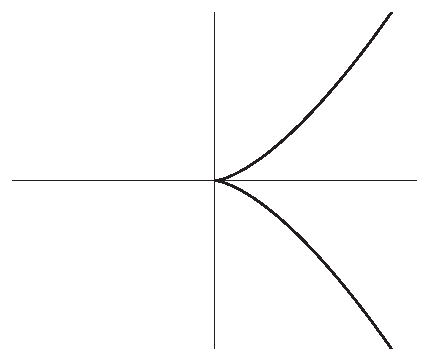
\includegraphics[width=5.0cm, natwidth=206mm, natheight=173mm]{/afs/athena.mit.edu/user/r/r/rrobinet/Documents/Github/18.721/images/Cusp/Cusp.pdf} \\
This is a nice caption.
\end{figure}

\begin{figure}[H]
\centering
\begin{examples}{}
\label{goober1}
\Marginnote{goober1}
\end{examples}
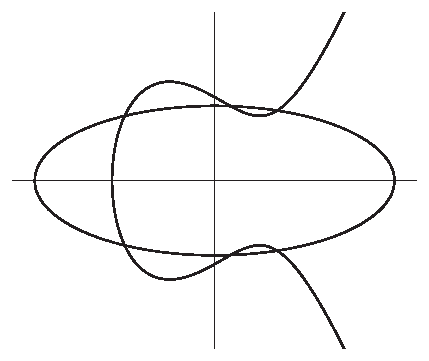
\includegraphics[width=5.0cm, natwidth=206mm, natheight=173mm]{/afs/athena.mit.edu/user/r/r/rrobinet/Documents/Github/18.721/images/Intersecting/Intersecting.pdf} \\
This is a nice caption.
\end{figure}

\begin{figure}[H]
\centering
\begin{examples}{}
\label{goober2}
\Marginnote{goober2}
\end{examples}
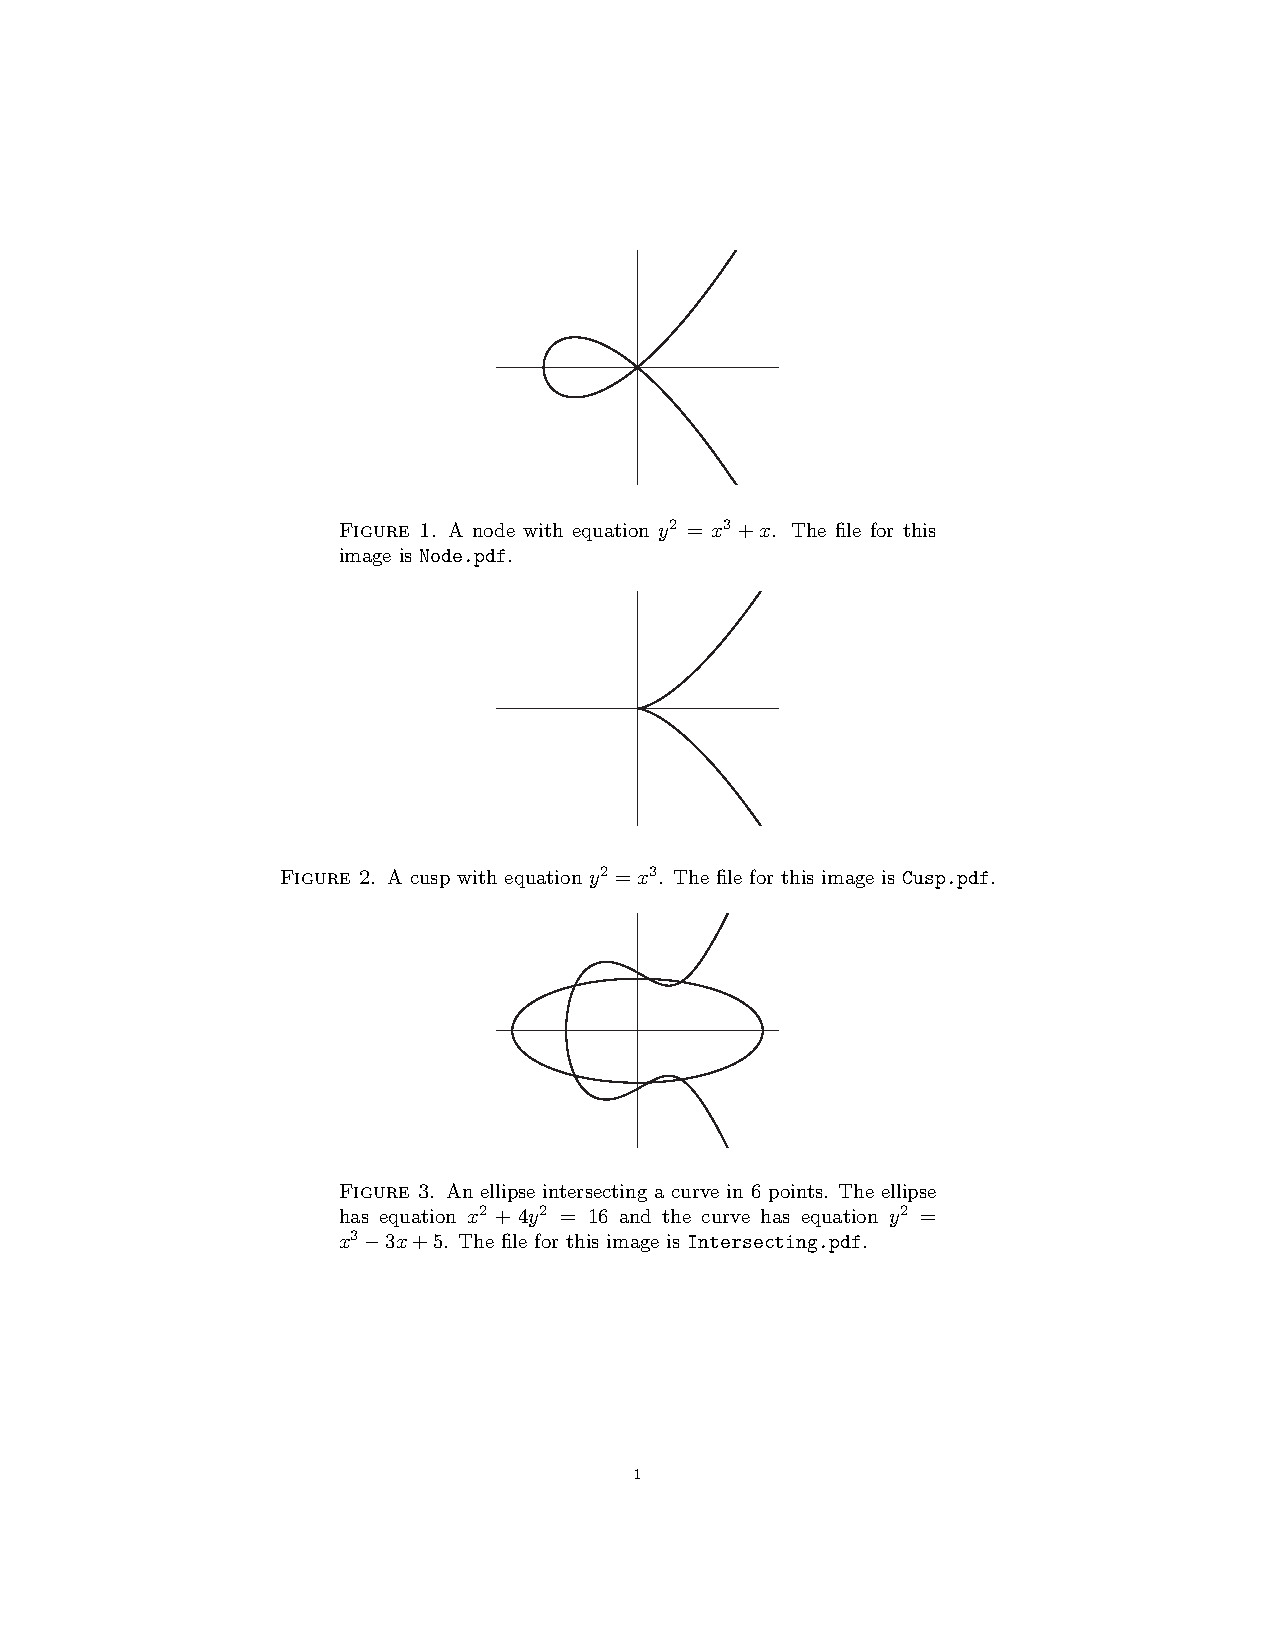
\includegraphics[width=5.0cm, natwidth=612mm, natheight=792mm]{/afs/athena.mit.edu/user/r/r/rrobinet/Documents/Github/18.721/images/Library/Library.pdf} \\
This is a nice caption.
\end{figure}

\begin{figure}[H]
\centering
\begin{examples}{}
\label{goober3}
\Marginnote{goober3}
\end{examples}
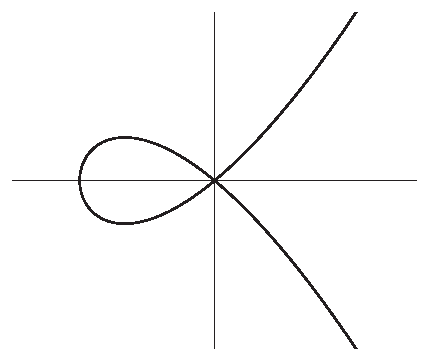
\includegraphics[width=5.0cm, natwidth=206mm, natheight=173mm]{/afs/athena.mit.edu/user/r/r/rrobinet/Documents/Github/18.721/images/Node/Node.pdf} \\
This is a nice caption.
\end{figure}

\begin{figure}[H]
\centering
\begin{examples}{}
\label{goober4}
\Marginnote{goober4}
\end{examples}
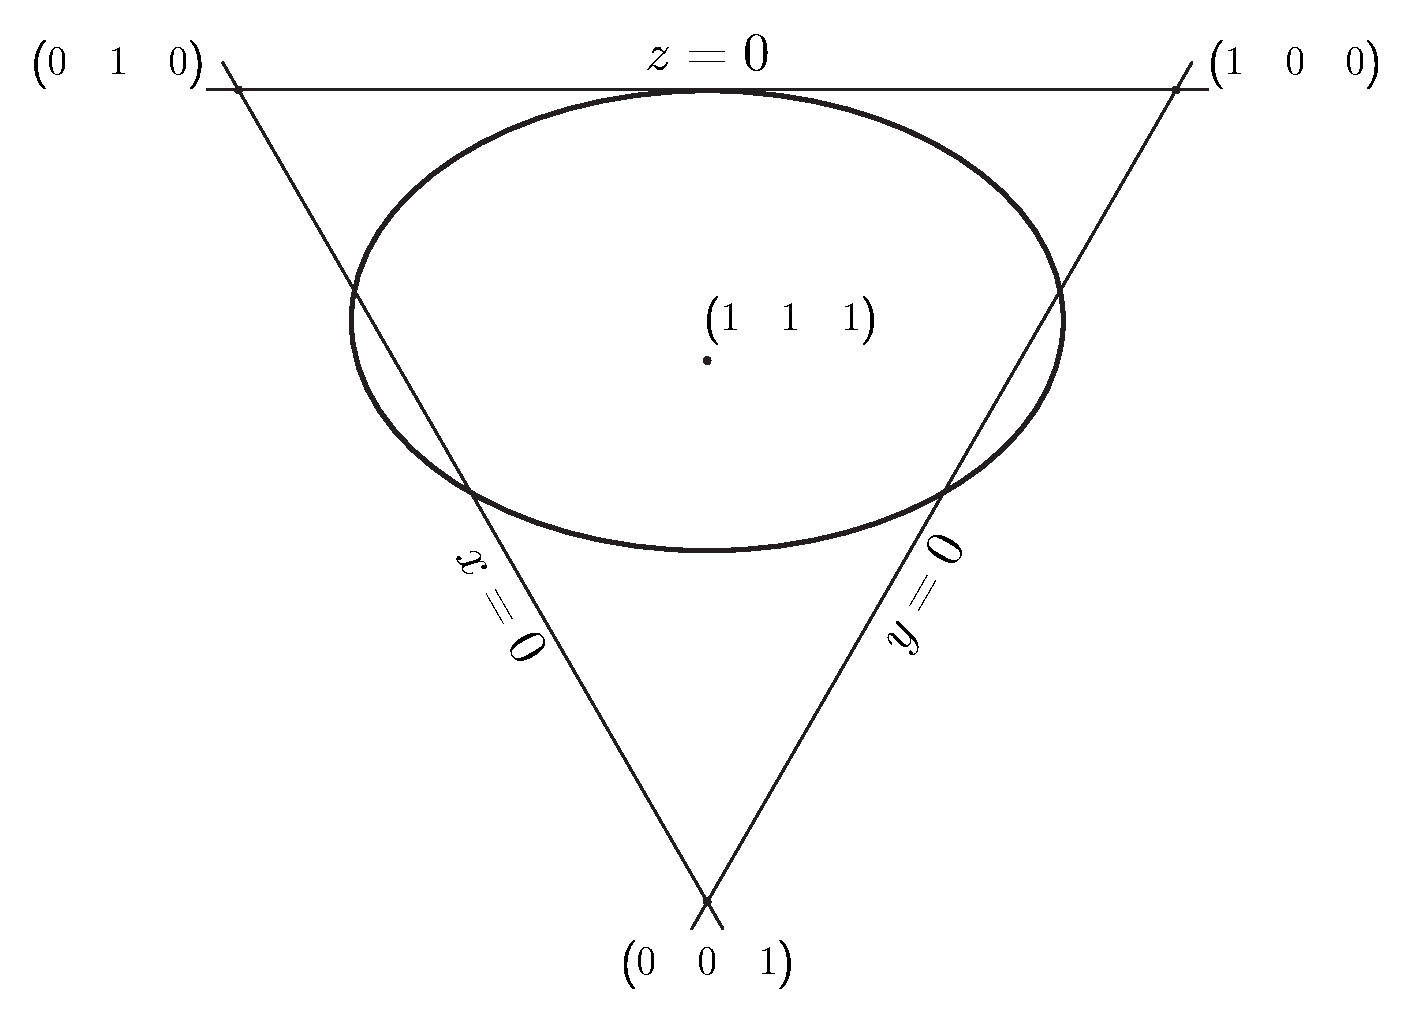
\includegraphics[width=5.0cm, natwidth=678mm, natheight=486mm]{/afs/athena.mit.edu/user/r/r/rrobinet/Documents/Github/18.721/images/Plane/Plane.pdf} \\
This is a nice caption.
\end{figure}

\begin{figure}[H]
\centering
\begin{examples}{}
\label{goober5}
\Marginnote{goober5}
\end{examples}
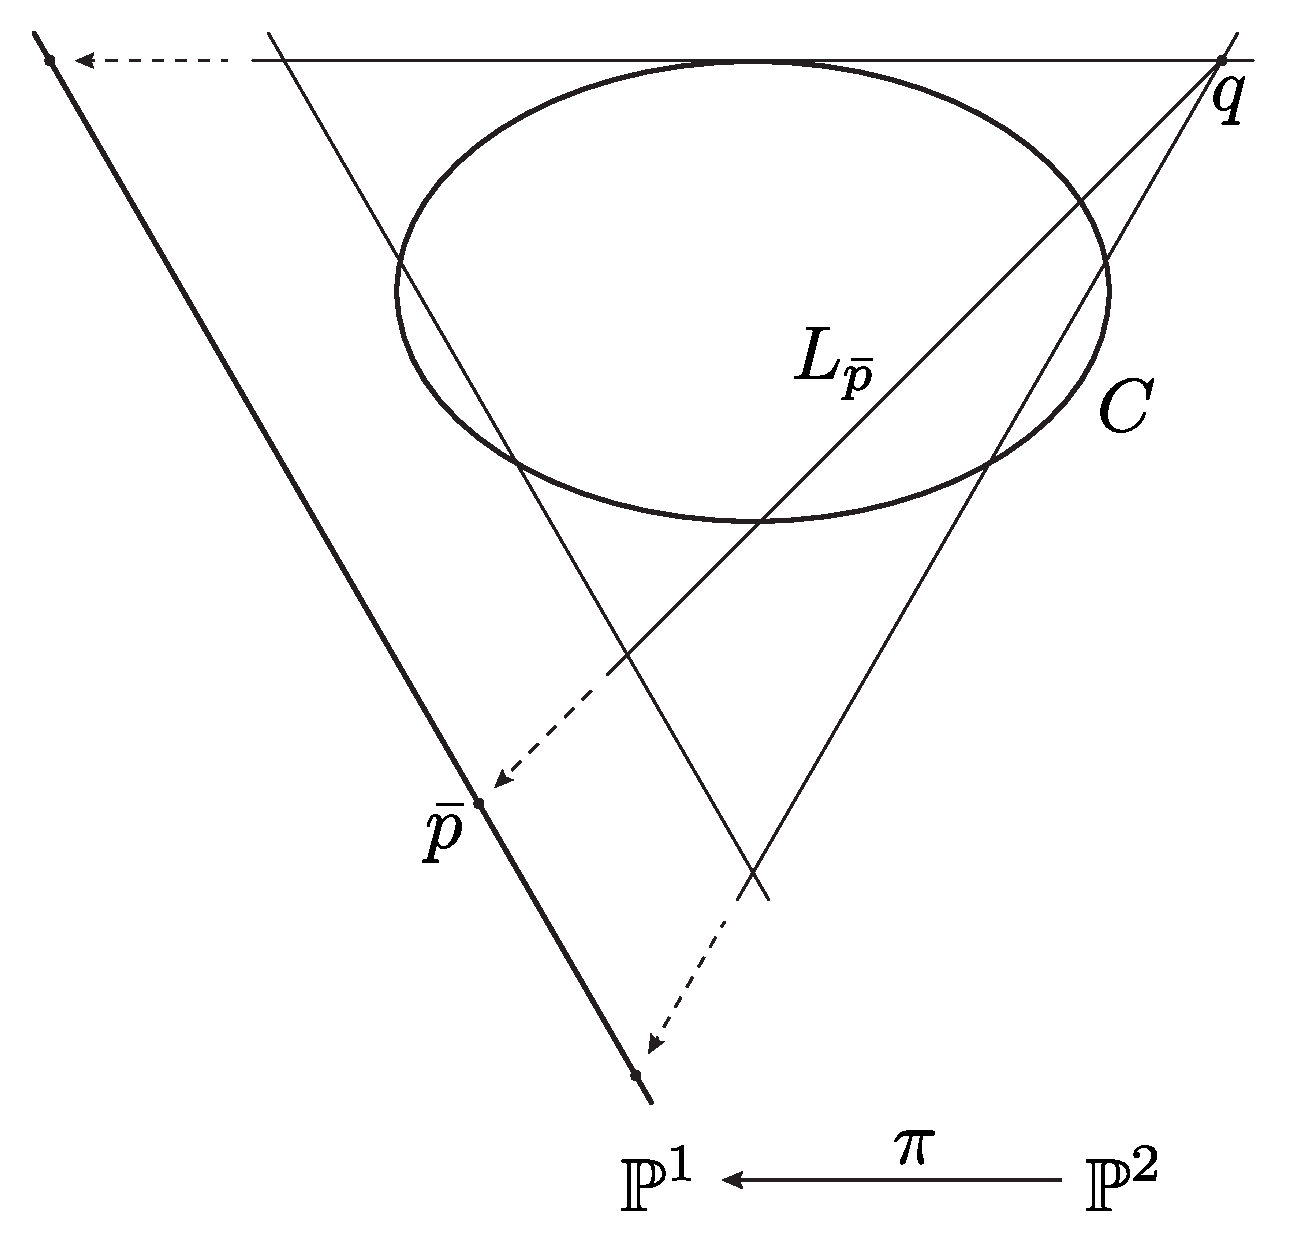
\includegraphics[width=5.0cm, natwidth=618mm, natheight=595mm]{/afs/athena.mit.edu/user/r/r/rrobinet/Documents/Github/18.721/images/Projecting/Projecting.pdf} \\
This is a nice caption.
\end{figure}

\begin{figure}[H]
\centering
\begin{examples}{}
\label{goober6}
\Marginnote{goober6}
\end{examples}
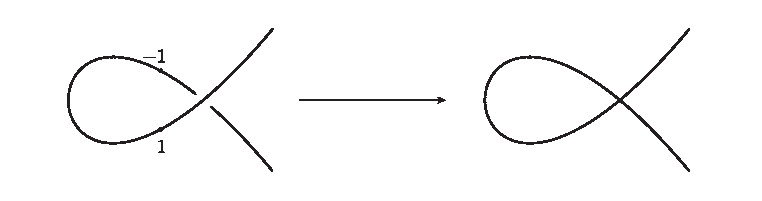
\includegraphics[width=5.0cm, natwidth=365mm, natheight=96mm]{/afs/athena.mit.edu/user/r/r/rrobinet/Documents/Github/18.721/images/projecting-node/project-node.pdf} \\
This is a nice caption.
\end{figure}

\begin{figure}[H]
\centering
\begin{examples}{}
\label{goober7}
\Marginnote{goober7}
\end{examples}
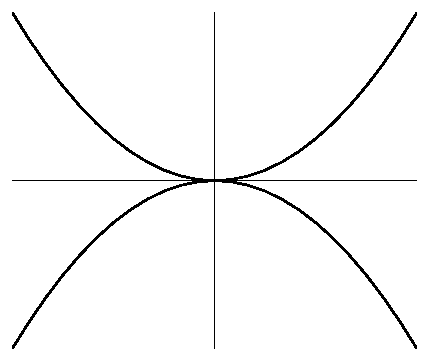
\includegraphics[width=5.0cm, natwidth=206mm, natheight=173mm]{/afs/athena.mit.edu/user/r/r/rrobinet/Documents/Github/18.721/images/tacnode/tacnode.pdf} \\
This is a nice caption.
\end{figure}

\begin{figure}[H]
\centering
\begin{examples}{}
\label{goober8}
\Marginnote{goober8}
\end{examples}
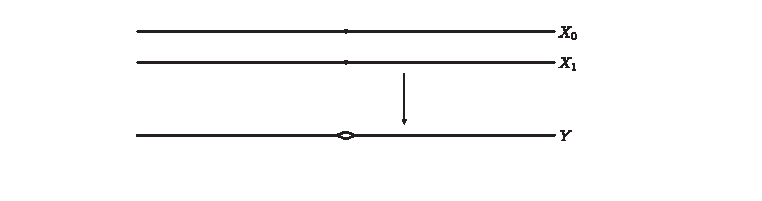
\includegraphics[width=5.0cm, natwidth=365mm, natheight=96mm]{/afs/athena.mit.edu/user/r/r/rrobinet/Documents/Github/18.721/images/two-origins/two-origins.pdf} \\
This is a nice caption.
\end{figure}

\begin{figure}[H]
\centering
\begin{examples}{}
\label{goober9}
\Marginnote{goober9}
\end{examples}
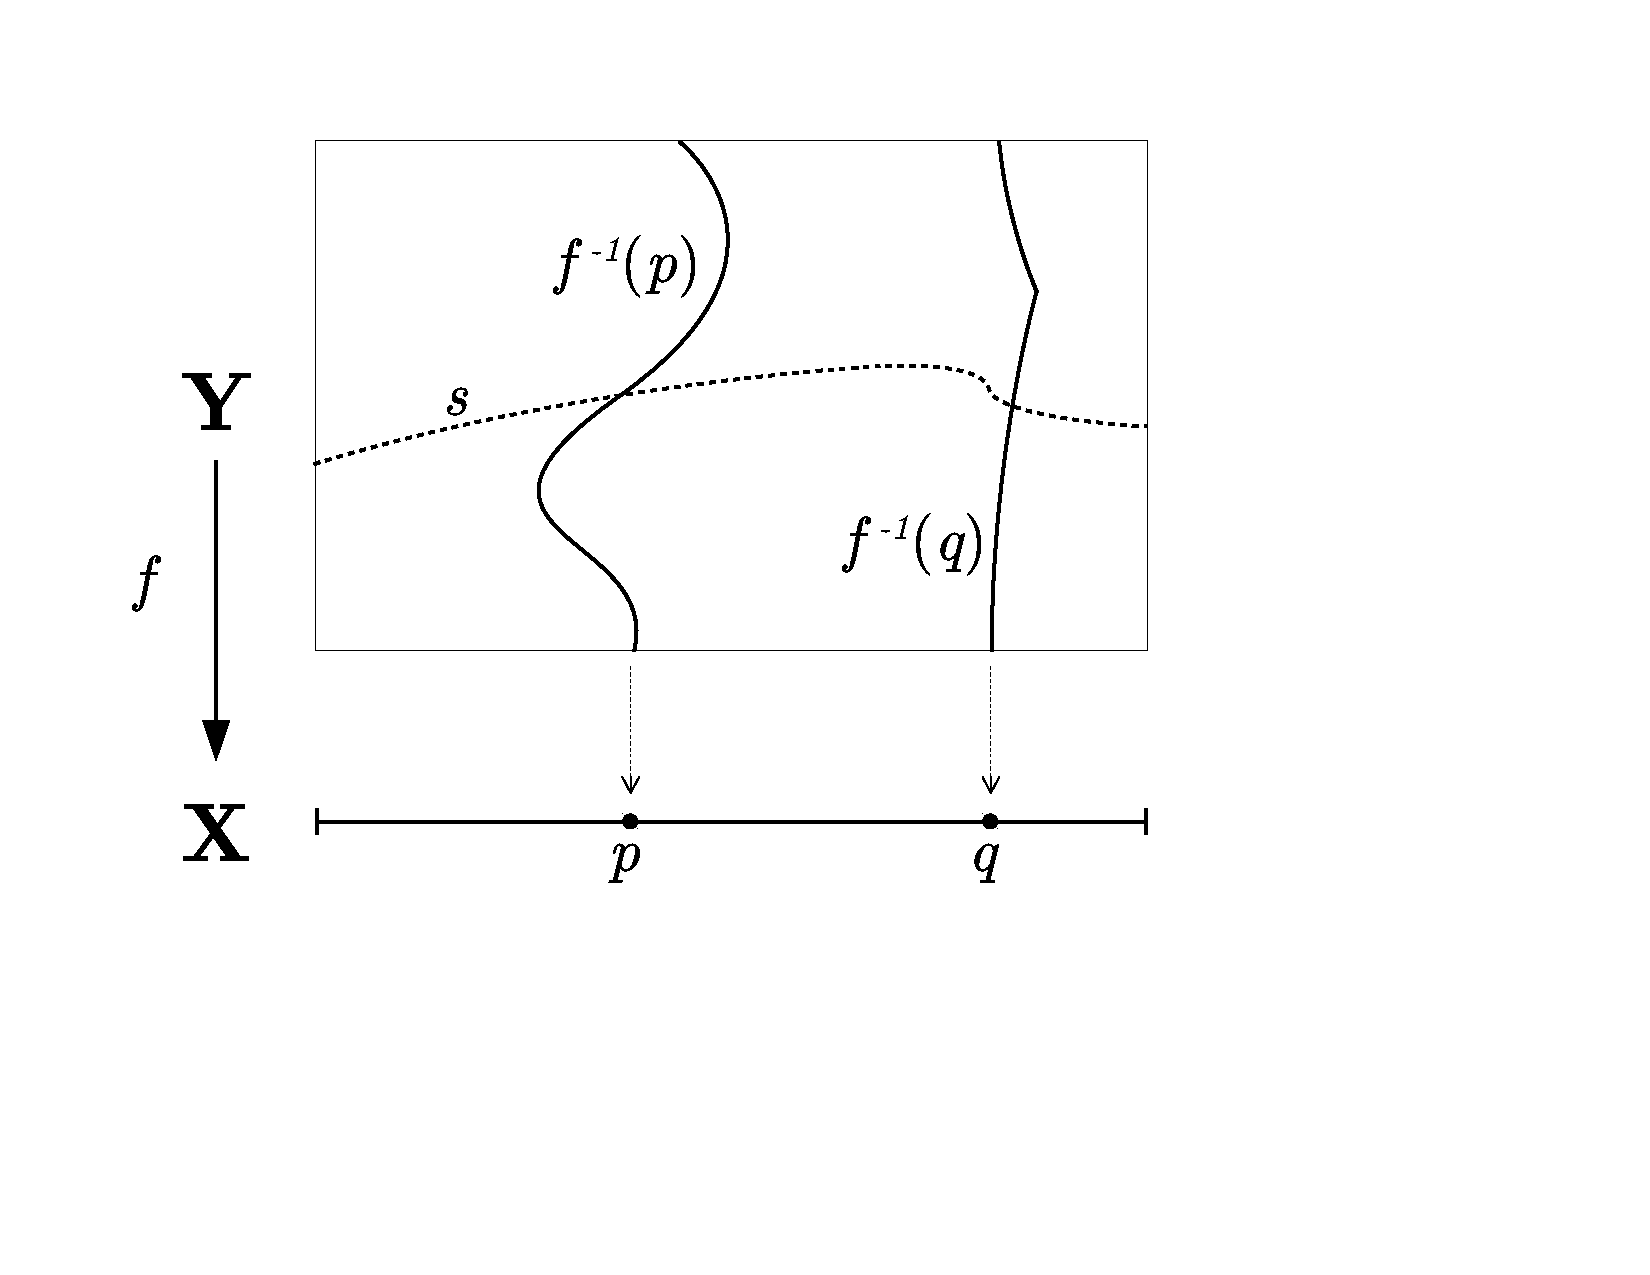
\includegraphics[width=5.0cm, natwidth=792mm, natheight=612mm]{/afs/athena.mit.edu/user/r/r/rrobinet/Documents/Github/18.721/images/my_figure/my_figure.pdf} \\
This is a nice caption.
\end{figure}

\begin{figure}[H]
\centering
\begin{examples}{}
\label{goober10}
\Marginnote{goober10}
\end{examples}
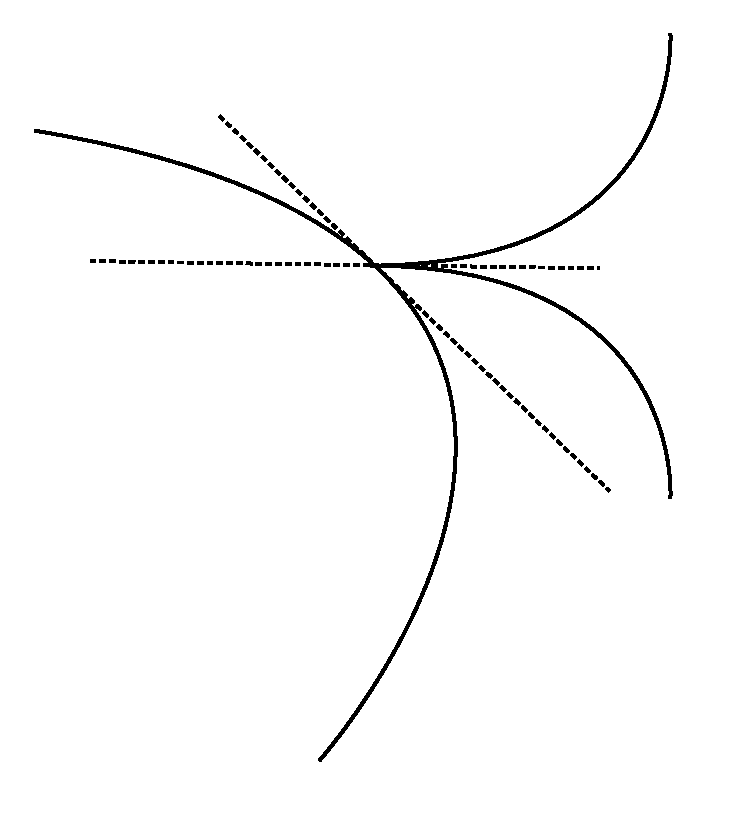
\includegraphics[width=5.0cm, natwidth=360mm, natheight=396mm]{/afs/athena.mit.edu/user/r/r/rrobinet/Documents/Github/18.721/images/intersxon_multi/intersxon_multi.pdf} \\
This is a nice caption.
\end{figure}

\begin{figure}[H]
\centering
\begin{examples}{}
\label{goober11}
\Marginnote{goober11}
\end{examples}
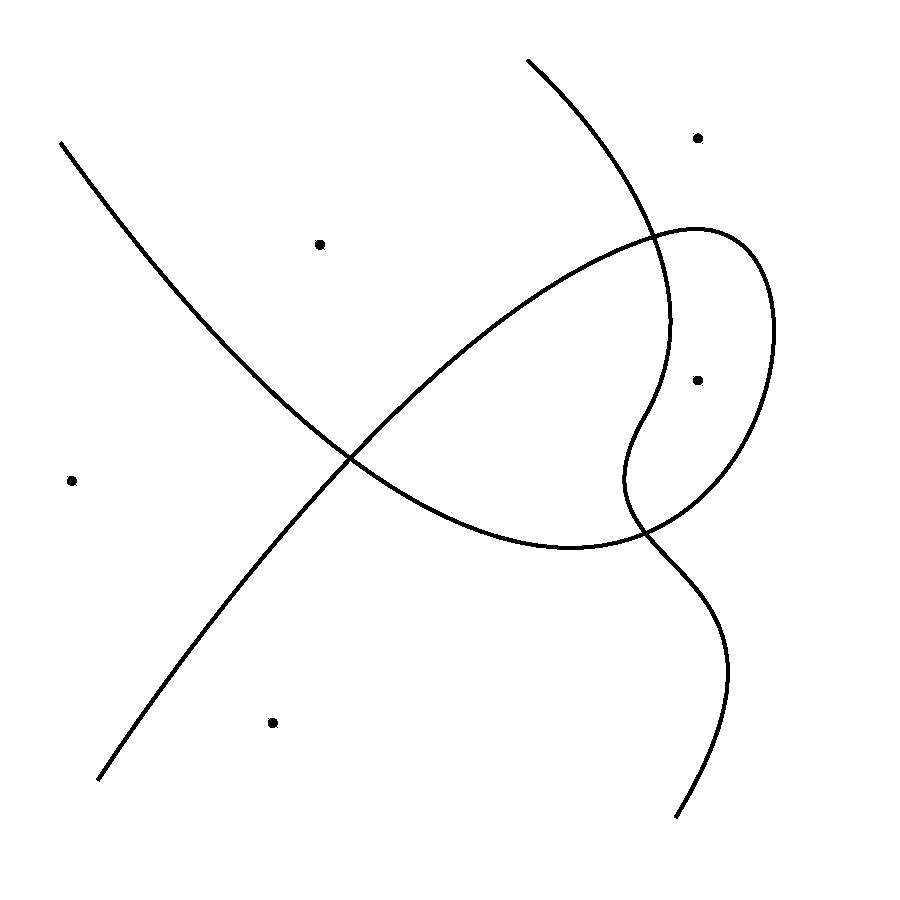
\includegraphics[width=5.0cm, natwidth=432mm, natheight=432mm]{/afs/athena.mit.edu/user/r/r/rrobinet/Documents/Github/18.721/images/zariski_closed/zariski_closed.pdf} \\
This is a nice caption.
\end{figure}

\begin{figure}[H]
\centering
\begin{examples}{}
\label{goober12}
\Marginnote{goober12}
\end{examples}
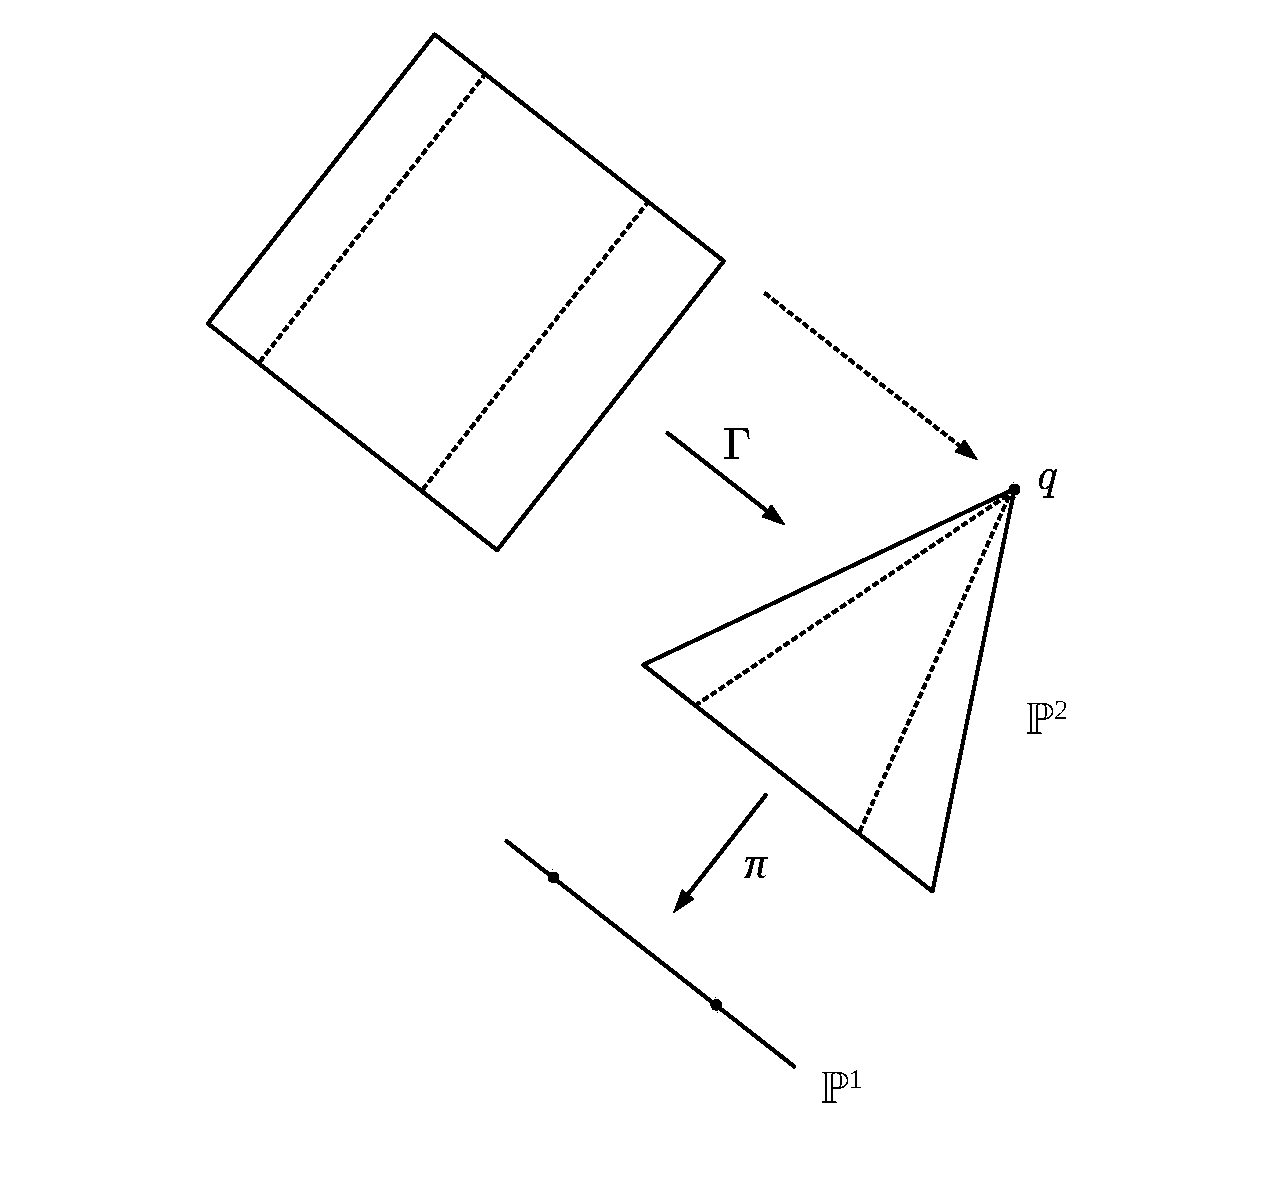
\includegraphics[width=5.0cm, natwidth=612mm, natheight=576mm]{/afs/athena.mit.edu/user/r/r/rrobinet/Documents/Github/18.721/images/proj_comp/proj_comp.pdf} \\
This is a nice caption.
\end{figure}

\begin{figure}[H]
\centering
\begin{examples}{}
\label{goober13}
\Marginnote{goober13}
\end{examples}
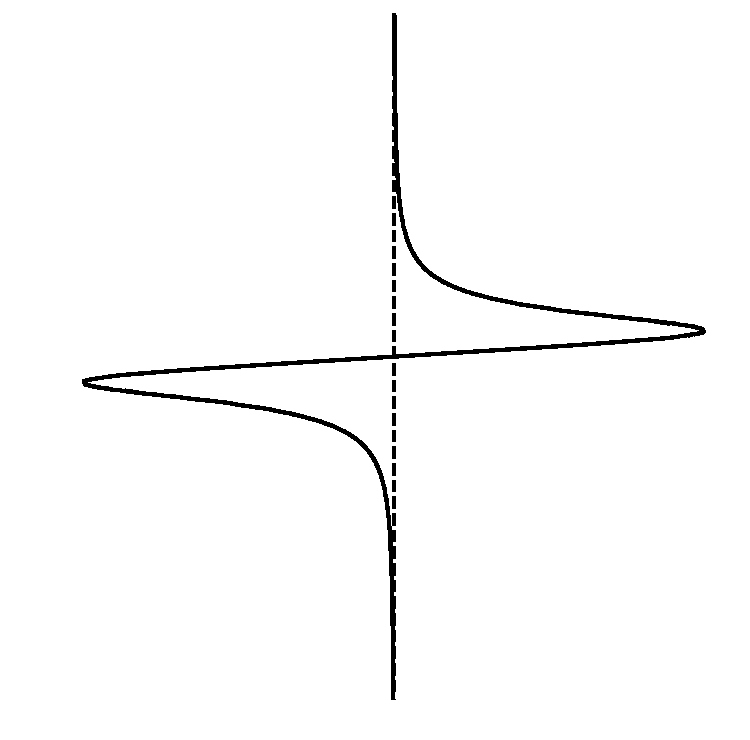
\includegraphics[width=5.0cm, natwidth=360mm, natheight=355mm]{/afs/athena.mit.edu/user/r/r/rrobinet/Documents/Github/18.721/images/Wolfram/asymptote.pdf} \\
This is a nice caption.
\end{figure}

\begin{figure}[H]
\centering
\begin{examples}{}
\label{goober14}
\Marginnote{goober14}
\end{examples}
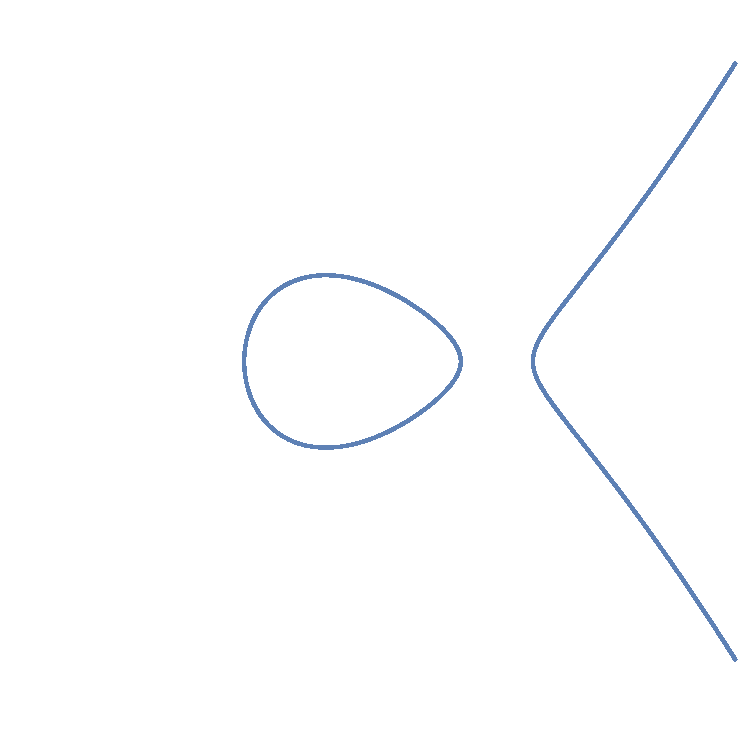
\includegraphics[width=5.0cm, natwidth=360mm, natheight=360mm]{/afs/athena.mit.edu/user/r/r/rrobinet/Documents/Github/18.721/images/Wolfram/cubic.pdf} \\
This is a nice caption.
\end{figure}

\begin{figure}[H]
\centering
\begin{examples}{}
\label{goober15}
\Marginnote{goober15}
\end{examples}
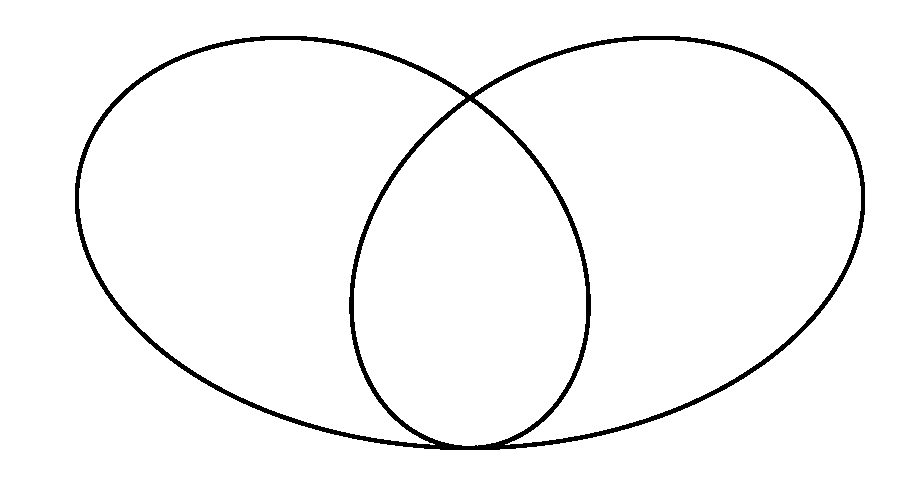
\includegraphics[width=5.0cm, natwidth=436mm, natheight=242mm]{/afs/athena.mit.edu/user/r/r/rrobinet/Documents/Github/18.721/images/Wolfram/capricornoid.pdf} \\
This is a nice caption.
\end{figure}

\begin{figure}[H]
\centering
\begin{examples}{}
\label{goober16}
\Marginnote{goober16}
\end{examples}
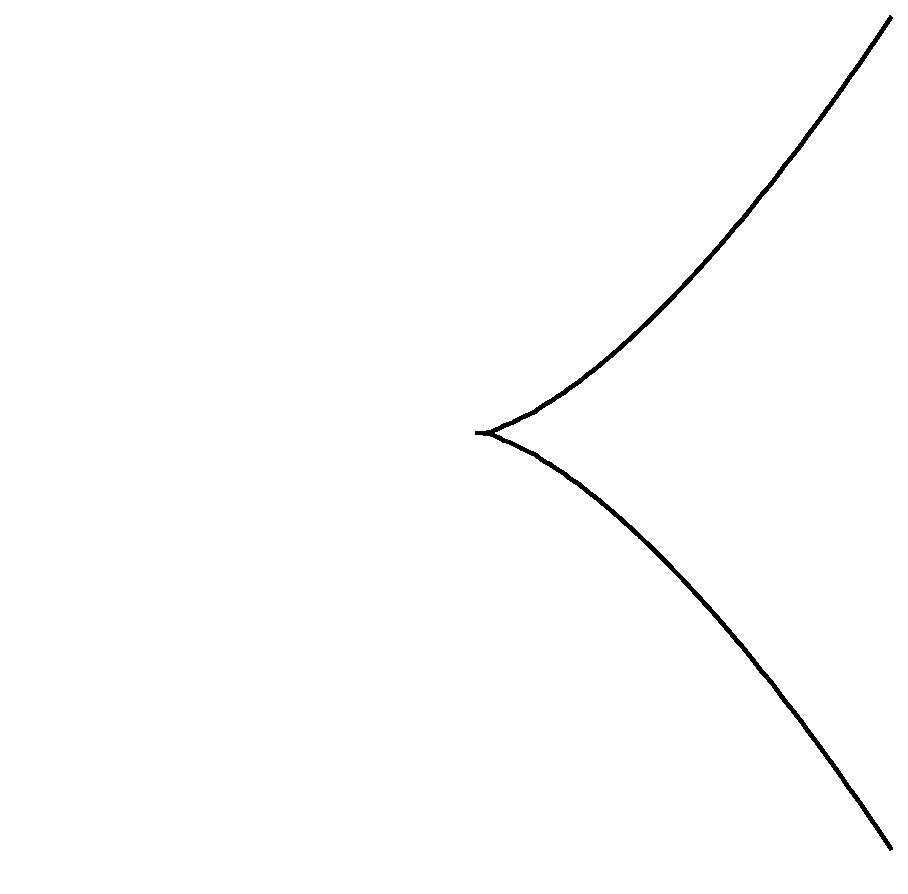
\includegraphics[width=5.0cm, natwidth=436mm, natheight=429mm]{/afs/athena.mit.edu/user/r/r/rrobinet/Documents/Github/18.721/images/Wolfram/parametrized_cusp.pdf} \\
This is a nice caption.
\end{figure}

\begin{figure}[H]
\centering
\begin{examples}{}
\label{goober17}
\Marginnote{goober17}
\end{examples}
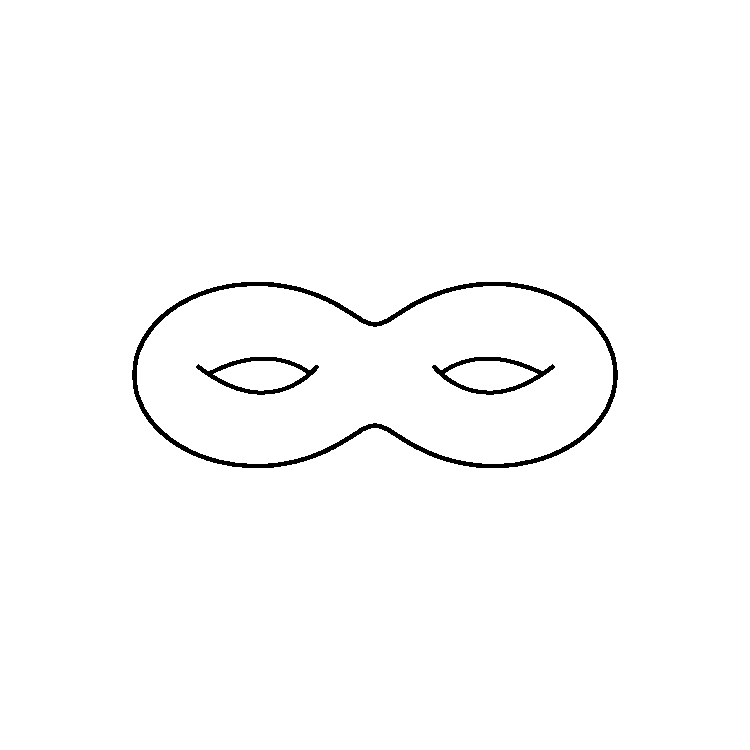
\includegraphics[width=5.0cm, natwidth=576mm, natheight=626mm]{/afs/athena.mit.edu/user/r/r/rrobinet/Documents/Github/18.721/images/Wolfram/double_torus.pdf} \\
This is a nice caption.
\end{figure}

\begin{figure}[H]
\centering
\begin{examples}{}
\label{goober18}
\Marginnote{goober18}
\end{examples}
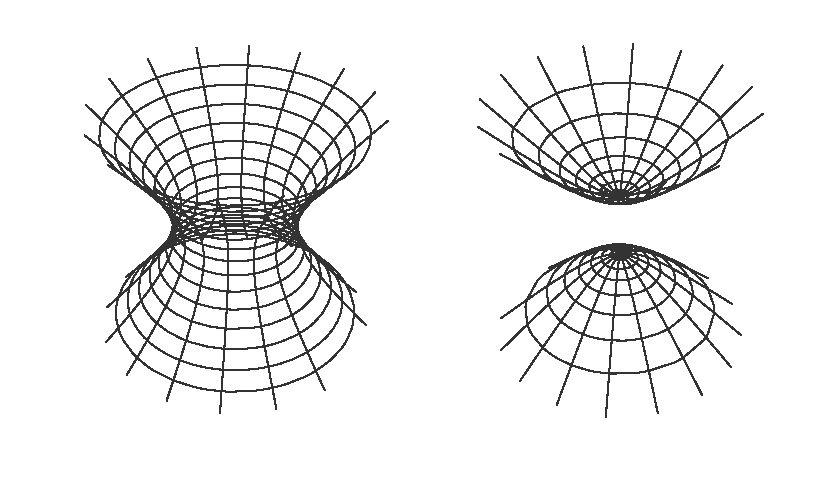
\includegraphics[width=5.0cm, natwidth=400mm, natheight=232mm]{/afs/athena.mit.edu/user/r/r/rrobinet/Documents/Github/18.721/images/Wolfram/ruled_hyperboloid.pdf} \\
This is a nice caption.
\end{figure}

\begin{figure}[H]
\centering
\begin{examples}{}
\label{goober19}
\Marginnote{goober19}
\end{examples}
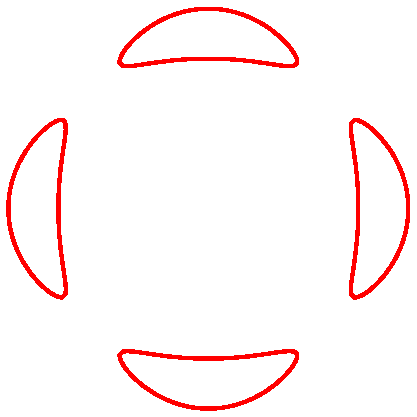
\includegraphics[width=5.0cm, natwidth=200mm, natheight=200mm]{/afs/athena.mit.edu/user/r/r/rrobinet/Documents/Github/18.721/images/Wolfram/trott_curve.pdf} \\
This is a nice caption.
\end{figure}

\begin{figure}[H]
\centering
\begin{examples}{}
\label{goober20}
\Marginnote{goober20}
\end{examples}
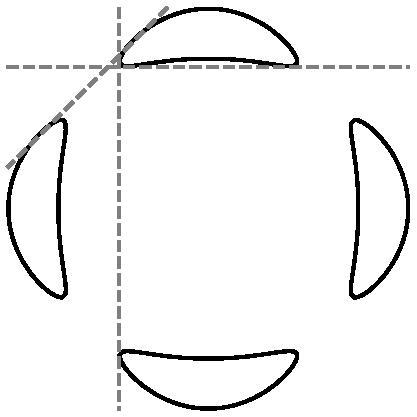
\includegraphics[width=5.0cm, natwidth=200mm, natheight=200mm]{/afs/athena.mit.edu/user/r/r/rrobinet/Documents/Github/18.721/images/Wolfram/trott_curve_tangents.pdf} \\
This is a nice caption.
\end{figure}

\end{document}
